\documentclass[12pt,a4paper]{article}
\usepackage[a4paper, margin=0.8in, headheight=14pt]{geometry}
\usepackage{fontspec}
\usepackage{unicode-math}
\setmainfont{TeX Gyre Pagella}
\setmonofont[Scale=0.88]{TeX Gyre Cursor}
\setmathfont{Latin Modern Math}
\usepackage{xcolor}
\usepackage{colortbl}
\usepackage{titlesec}
\usepackage{enumitem}
\usepackage{tabularx}
\usepackage{booktabs}
\usepackage{array}
\usepackage{amsmath}
\usepackage{tikz}
\usetikzlibrary{shapes.geometric, arrows.meta, positioning, calc, fit, decorations.pathreplacing, decorations.pathmorphing, patterns}
\usepackage[american]{circuitikz}
\usepackage{tcolorbox}
\tcbuselibrary{skins, breakable}
\usepackage{hyperref}
\usepackage{fancyhdr}
\usepackage{graphicx}
\usepackage{microtype}
\hyphenpenalty=10000
\exhyphenpenalty=10000
\sloppy
\usepackage{caption}
\usepackage{setspace}
\usepackage{multirow}
\usepackage{tocloft}
\newcommand{\Q}[1]{\textbf{#1}\par\noindent\ignorespaces}
\definecolor{myred}{RGB}{196,30,58}
\definecolor{mydark}{RGB}{30,30,50}
\definecolor{mygreen}{RGB}{14,120,80}
\definecolor{myteal}{RGB}{0,130,140}
\definecolor{myamber}{RGB}{180,100,0}
\definecolor{mypurple}{RGB}{100,30,160}
\definecolor{mygray}{RGB}{246,247,249}
\definecolor{mgframe}{RGB}{180,185,200}
\definecolor{watermark}{RGB}{145,150,170}
\definecolor{hdrred}{RGB}{250,232,235}
\definecolor{hdrgreen}{RGB}{220,244,233}
\definecolor{hdrteal}{RGB}{220,242,244}
\definecolor{hdramber}{RGB}{253,242,215}
\definecolor{hdrpurple}{RGB}{238,228,255}
\definecolor{hdrgray}{RGB}{238,240,245}
\definecolor{rowalt}{RGB}{250,251,253}

\titleformat{\section}{\large\bfseries\color{myred}}{\thesection.}{0.5em}{}[\vspace{1pt}{\color{myred}\rule{\linewidth}{0.8pt}}]
\titleformat{\subsection}{\normalsize\bfseries\color{myteal}}{\thesubsection}{0.5em}{}
\titlespacing*{\section}{0pt}{18pt}{7pt}
\titlespacing*{\subsection}{0pt}{11pt}{4pt}
\setlength{\parindent}{0pt}
\setlength{\parskip}{4pt}
\renewcommand{\cfttoctitlefont}{\large\bfseries\color{myred}}
\renewcommand{\cftaftertoctitle}{\par\noindent{\color{myred}\rule{\linewidth}{0.8pt}}}
\setlength{\cftbeforetoctitleskip}{0pt}
\setlength{\cftaftertoctitleskip}{6pt}
\renewcommand{\cftsecfont}{\normalsize\bfseries\color{mydark}}
\renewcommand{\cftsecpagefont}{\normalsize\bfseries\color{mydark}}
\renewcommand{\cftsecleader}{\cftdotfill{\cftdotsep}}
\setlength{\cftbeforesecskip}{7pt}
\renewcommand{\cftsubsecfont}{\small\color{mydark}}
\renewcommand{\cftsubsecpagefont}{\small\color{mydark}}
\setlength{\cftbeforesubsecskip}{3pt}
\setlength{\cftsubsecindent}{1.4em}
\renewcommand{\cftpartfont}{\normalsize\bfseries\color{myteal}}
\renewcommand{\cftpartpagefont}{\normalsize\bfseries\color{myteal}}
\setlength{\cftbeforepartskip}{14pt}
\renewcommand{\arraystretch}{1.45}
\setlength{\tabcolsep}{6pt}
\arrayrulecolor{mydark}
\newcolumntype{B}[1]{>{\small\bfseries\raggedright\arraybackslash}m{#1}}
\newcolumntype{C}[1]{>{\centering\arraybackslash}m{#1}}
\newcolumntype{Y}{>{\small\raggedright\arraybackslash}X}
\renewcommand{\tabularxcolumn}[1]{m{#1}}
\newcommand{\currmodule}{Module 1}
\pagestyle{fancy}
\fancyhf{}
\fancyhead[L]{\small\color{myred}\textbf{PE-EC603B}\;\color{mydark}--- Bio-Medical Electronics}
\fancyhead[R]{\small\color{myteal}\textbf{\currmodule\ Notes}}
\fancyfoot[C]{\small\color{mydark}\thepage}
\fancyfoot[R]{\small\color{watermark}\textit{\copyright\ Biraj}}
\renewcommand{\headrulewidth}{0.5pt}
\renewcommand{\footrulewidth}{0.3pt}

\hypersetup{colorlinks=true, linkcolor=myteal, urlcolor=myteal,
  pdfauthor={Biraj Sarkar},
  pdftitle={PE-EC603B --- Combined Notes}}

\tcbset{
  tikzbox/.style={
    colback=mygray, colframe=mgframe, boxrule=0.6pt, arc=4pt,
    left=8pt, right=8pt, top=6pt, bottom=6pt,
    colbacktitle=mgframe, coltitle=mydark,
    fonttitle=\small\bfseries
  },
  defbox/.style={
    colback=hdrgreen, colframe=mygreen, boxrule=0.8pt, arc=4pt,
    left=9pt, right=9pt, top=6pt, bottom=6pt,
    colbacktitle=mygreen, coltitle=white,
    fonttitle=\small\bfseries
  },
  formulabox/.style={
    colback=hdrteal, colframe=myteal, boxrule=0.8pt, arc=4pt,
    left=9pt, right=9pt, top=7pt, bottom=7pt,
    colbacktitle=myteal, coltitle=white,
    fonttitle=\small\bfseries
  },
  examplebox/.style={
    colback=hdramber, colframe=myamber, boxrule=0.8pt, arc=4pt,
    left=9pt, right=9pt, top=6pt, bottom=6pt,
    colbacktitle=myamber, coltitle=white,
    fonttitle=\small\bfseries
  },
  masonbox/.style={
    colback=hdrpurple, colframe=mypurple, boxrule=0.8pt, arc=4pt,
    left=9pt, right=9pt, top=6pt, bottom=6pt,
    colbacktitle=mypurple, coltitle=white,
    fonttitle=\small\bfseries
  },
  exambox/.style={
    colback=hdrpurple, colframe=mypurple, boxrule=1pt, arc=5pt,
    left=10pt, right=10pt, top=8pt, bottom=8pt,
    colbacktitle=mypurple, coltitle=white,
    fonttitle=\bfseries,
    breakable, title after break={\textbf{Frequently Asked / Viva Questions (contd.)}}}
}
\tcbset{breakable}
\tcbset{after={\color{black}}}

\tikzset{
  block/.style={rectangle, draw=myteal, fill=hdrteal,
    text width=2.4cm, align=center, minimum height=0.95cm,
    font=\small, rounded corners=3pt, line width=0.7pt},
  redblock/.style={rectangle, draw=myred, fill=hdrred,
    text width=2.4cm, align=center, minimum height=0.95cm,
    font=\small, rounded corners=3pt, line width=0.7pt},
  greenblock/.style={rectangle, draw=mygreen, fill=hdrgreen,
    text width=2.4cm, align=center, minimum height=0.95cm,
    font=\small, rounded corners=3pt, line width=0.7pt},
  amberblock/.style={rectangle, draw=myamber, fill=hdramber,
    text width=2.4cm, align=center, minimum height=0.95cm,
    font=\small, rounded corners=3pt, line width=0.7pt},
  purpblock/.style={rectangle, draw=mypurple, fill=hdrpurple,
    text width=2.4cm, align=center, minimum height=0.95cm,
    font=\small, rounded corners=3pt, line width=0.7pt},
  sumjunc/.style={circle, draw=myamber, fill=hdramber,
    minimum size=0.62cm, font=\small, line width=0.8pt},
  arrow/.style={-Stealth, thick, color=mydark},
  redarrow/.style={-Stealth, thick, color=myred},
  line/.style={thick, color=mydark}
}

\newcommand{\modulestart}[2]{%
  \clearpage
  \renewcommand{\currmodule}{Module #1}%
  \renewcommand{\theHsection}{mod#1.\arabic{section}}%
  \renewcommand{\theHsubsection}{\theHsection.\arabic{subsection}}%
  \renewcommand{\theHsubsubsection}{\theHsubsection.\arabic{subsubsection}}%
  \phantomsection
  \addcontentsline{toc}{part}{Module #1: #2}%
  \setcounter{section}{0}%
  \begin{center}
    \vspace*{1.0cm}
    {\Huge\bfseries\color{myred} Module #1}\\[10pt]
    {\Large\bfseries\color{mydark} #2}\\[10pt]
    {\color{myred}\rule{0.55\linewidth}{1.2pt}}
  \end{center}
  \vspace{14pt}
}
\begin{document}

\thispagestyle{empty}

% ─── Page Border (TikZ Overlay) ────────────────────────────────────────────────
\begin{tikzpicture}[remember picture, overlay]
  % Outer border (fine line in mgframe)
  \draw[color=mgframe, line width=1.5pt] 
    ($(current page.north west) + (0.6in, -0.6in)$) rectangle 
    ($(current page.south east) + (-0.6in, 0.6in)$);
  % Inner border (finer accent line in myred)
  \draw[color=myred, line width=0.8pt] 
    ($(current page.north west) + (0.65in, -0.65in)$) rectangle 
    ($(current page.south east) + (-0.65in, 0.65in)$);
\end{tikzpicture}

\vspace*{1.0cm}
\begin{center}
  {\Huge\bfseries\color{myred} PE-EC603B}\\[10pt]
  {\LARGE\bfseries\color{mydark} Bio-Medical Electronics}\\[20pt]
  {\color{myred}\rule{0.7\linewidth}{1.5pt}}\\[18pt]
  {\Large\color{myteal}\textbf{Combined Module Notes}}\\[8pt]
  {\large\color{mydark} Modules 1 -- 4}\\[40pt]
  {\normalsize\color{mydark} Semester VI \quad$\bullet$\quad ECE \quad$\bullet$\quad 3 Credits}\\[12pt]
  {\normalsize\color{mydark} CGEC \;$|$\; B.Tech ECE (2023--27)}
\end{center}
\vspace{1.0cm}
\begin{center}
  \begin{tcolorbox}[colback=mygray, colframe=mgframe, boxrule=0.5pt, arc=3pt, width=0.85\linewidth]
    \centering\small\color{mydark}
    \textbf{Disclaimer / Study Guide Notice:}\\
    These are condensed \textbf{Short Notes} focusing on core theory, key formulas, block/circuit diagrams, and standard viva Q\&As for university exam revision. Exhaustive numerical practice problems and derivation edge cases are not covered. This serves as a quick-revision reference guide for students.
  \end{tcolorbox}
\end{center}
\vfill
\vspace{0.6cm}
\begin{center}
  {\large\bfseries\color{mypurple} Biraj Sarkar}\\[16pt]
  {\footnotesize\color{watermark}\textbf{IN ASSOCIATION WITH}}\\[8pt]
  {\small\bfseries\color{mydark} MAKAUT Wingman \quad$\bullet$\quad MAKAUT Future Minds}\\[12pt]
  {\large\bfseries\color{myteal} Cooch Behar Government Engineering College}
\end{center}
\vfill
\begin{center}{\small\color{watermark}\textit{Exam-Ready Notes}}\end{center}
\clearpage

\hypersetup{linkcolor=mydark}
\tableofcontents
\hypersetup{linkcolor=myteal}
\clearpage

% -- Module 1 -----------------------------------------------------------------
\modulestart{1}{The Human Body as an Engineering System}

\section{The Human Body as an Engineering System}
% ===============================================================================

The human body can be viewed as a highly complex, self-regulating biological machine. From a bio-medical electronics perspective, it is a system with sensors (sense organs), processors (nervous system and brain), actuators (muscles), and a power supply (metabolic energy from food). Understanding this system is essential for designing instruments that measure, monitor, and assist bodily functions.

\subsection{Organ Systems Overview}

\begin{tcolorbox}[defbox, title={\textbf{Definition: Organ System}}]
An \textbf{organ system} is a group of organs that work together to perform one or more physiological functions. The human body consists of 11 major organ systems, each with specific roles in maintaining homeostasis.
\end{tcolorbox}

\textbf{Major Organ Systems Relevant to Bio-Medical Electronics:}\par\noindent
\begin{tabularx}{\linewidth}{|B{3.2cm}|Y|Y|}
\hline
\textbf{System} & \textbf{\color{myteal}Primary Organs} & \textbf{\color{mygreen}Clinical Relevance} \\
\hline
\textbf{Cardiovascular} & Heart, arteries, veins, capillaries. & ECG, blood pressure, cardiac output monitoring. \\
\hline
\textbf{Respiratory} & Lungs, diaphragm, trachea, bronchi. & Spirometry, pulse oximetry, ventilator design. \\
\hline
\textbf{Nervous} & Brain, spinal cord, peripheral nerves. & EEG, EMG, nerve conduction velocity. \\
\hline
\textbf{Muscular} & Skeletal, smooth, cardiac muscle. & EMG, prosthetic limb control, physiotherapy. \\
\hline
\textbf{Renal (Urinary)} & Kidneys, ureter, bladder. & Dialysis machine design, fluid balance monitoring. \\
\hline
\textbf{Endocrine} & Pancreas, thyroid, adrenal glands. & Blood glucose monitoring, hormone assay. \\
\hline
\end{tabularx}

\subsection{Homeostasis and Feedback Control}

\begin{tcolorbox}[defbox, title={\textbf{Definition: Homeostasis}}]
\textbf{Homeostasis} is the ability of a living organism to maintain a stable internal environment despite changes in external conditions. It is achieved through continuous negative feedback loops involving sensors, control centers, and effectors.
\end{tcolorbox}

The body maintains homeostasis by regulating parameters such as body temperature ($37\pm0.5\,^{\circ}\text{C}$), blood pH ($7.35$--$7.45$), blood glucose ($70$--$100\,\text{mg/dL}$), and arterial blood pressure ($120/80\,\text{mmHg}$). Most clinical instruments are designed to monitor deviations from these normal (baseline) values.

\begin{tcolorbox}[tikzbox, title={Biological Feedback Control Loop (Homeostasis)}]
\centering
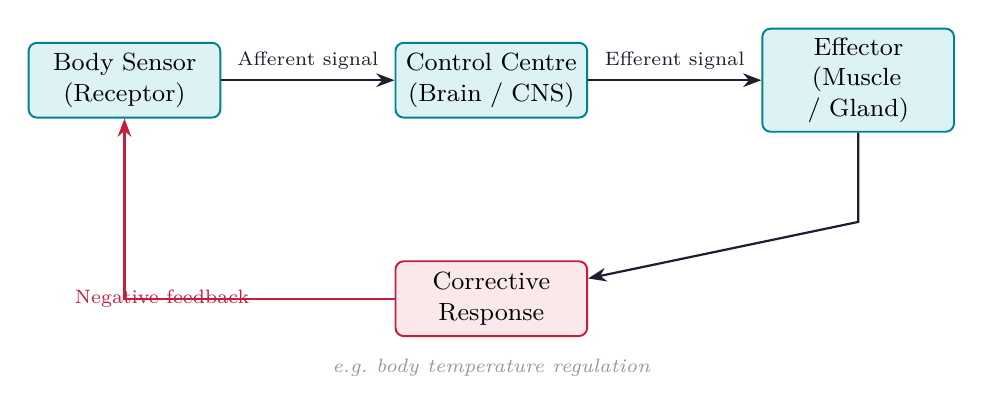
\begin{tikzpicture}[node distance=1.1cm and 2.0cm, thick]
  \node[block, text width=2.2cm] (sensor) {Body Sensor\\(Receptor)};
  \node[block, text width=2.2cm, right=2.2cm of sensor] (control) {Control Centre\\(Brain / CNS)};
  \node[block, text width=2.2cm, right=2.2cm of control] (effector) {Effector\\(Muscle / Gland)};
  \node[redblock, text width=2.2cm, below=1.8cm of control] (response) {Corrective\\Response};

  \draw[arrow] (sensor) -- node[above, font=\scriptsize, color=mydark] {Afferent signal} (control);
  \draw[arrow] (control) -- node[above, font=\scriptsize, color=mydark] {Efferent signal} (effector);
  \draw[arrow] (effector) -- ++(0,-1.8) -- (response);
  \draw[redarrow] (response) -- node[left, font=\scriptsize, color=myred] {Negative feedback} (sensor |- response) -- (sensor);

  \node[font=\scriptsize\itshape, color=watermark, below=0.15cm of response] {e.g.\ body temperature regulation};
\end{tikzpicture}
\end{tcolorbox}

% ===============================================================================
\section{The Cardiovascular System}
% ===============================================================================

The cardiovascular system (CVS) is the most extensively monitored system in bio-medical electronics, since the heart generates measurable electrical, pressure, and acoustic signals accessible from the body surface.

\subsection{Structure and Function}

\begin{tcolorbox}[defbox, title={\textbf{Definition: Cardiovascular System}}]
The \textbf{cardiovascular system} consists of the heart (pump), blood vessels (conduits), and blood (transport medium). It delivers oxygen, nutrients, and hormones to all tissues and removes metabolic waste products.
\end{tcolorbox}

The heart is a four-chambered muscular pump:
\begin{itemize}[leftmargin=*, itemsep=3pt]
  \item \textbf{Right Atrium (RA):} Receives deoxygenated blood from the body via the superior and inferior vena cava.
  \item \textbf{Right Ventricle (RV):} Pumps blood to the lungs through the pulmonary artery (pulmonary circulation).
  \item \textbf{Left Atrium (LA):} Receives oxygenated blood from the lungs via pulmonary veins.
  \item \textbf{Left Ventricle (LV):} Pumps oxygenated blood to the entire body through the aorta (systemic circulation). The LV wall is thickest because it works against the highest pressure.
\end{itemize}

\subsection{The Cardiac Cycle and Electrical Conduction}

Each heartbeat is initiated by the \textbf{Sinoatrial (SA) node} --- the heart's natural pacemaker located in the right atrium. The electrical impulse propagates through a defined conduction pathway:

\textbf{SA Node $\to$ AV Node $\to$ Bundle of His $\to$ Left and Right Bundle Branches $\to$ Purkinje Fibres $\to$ Ventricular Myocardium}

\begin{tcolorbox}[formulabox, title={\textbf{Cardiovascular Parameters and Normal Values}}]
\renewcommand{\arraystretch}{1.3}
\begin{tabularx}{\linewidth}{B{3.8cm} X}
Heart Rate (HR) & $60$--$100\,\text{beats/min}$ (normal); $< 60$ = bradycardia; $> 100$ = tachycardia. \\[4pt]
Stroke Volume (SV) & Volume ejected per beat $\approx 70\,\text{mL}$ at rest. \\[4pt]
Cardiac Output (CO) & $CO = HR \times SV \approx 5\,\text{L/min}$ at rest. \\[4pt]
Blood Pressure (BP) & Systolic $\approx 120\,\text{mmHg}$; Diastolic $\approx 80\,\text{mmHg}$. \\[4pt]
Mean Arterial Pressure & $MAP = \displaystyle\frac{SBP + 2 \times DBP}{3} \approx 93\,\text{mmHg}$.
\end{tabularx}
\end{tcolorbox}

\subsection{The ECG Signal}

The electrocardiogram (ECG) is a recording of the electrical activity of the heart from the body surface. Each cardiac cycle produces a characteristic waveform:

\begin{tcolorbox}[tikzbox, title={ECG Waveform --- Components and Significance}]
\centering
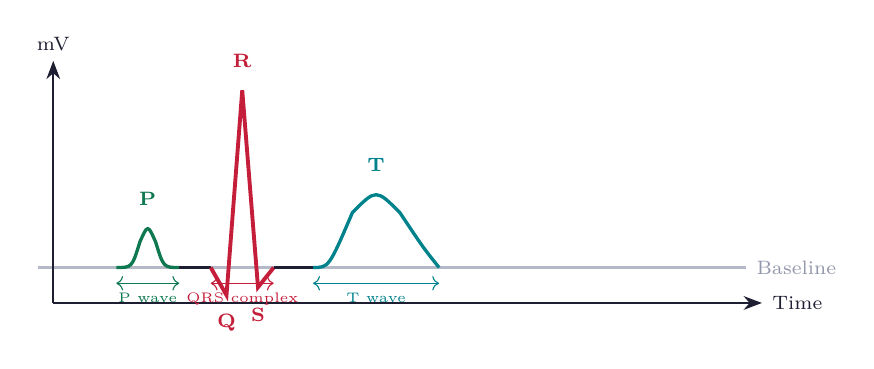
\begin{tikzpicture}[x=1.0cm, y=2.5cm, thick]
  % Baseline
  \draw[line, color=mgframe] (-0.5, 0) -- (8.5, 0) node[right, font=\scriptsize, color=watermark] {Baseline};
  % Time axis
  \draw[arrow] (-0.3, -0.18) -- (8.7, -0.18) node[right, font=\scriptsize] {Time};
  % Voltage axis
  \draw[arrow] (-0.3, -0.18) -- (-0.3, 1.05) node[above, font=\scriptsize] {mV};

  % P wave (small positive hump)
  \draw[color=mygreen, line width=1.2pt]
    (0.5, 0) .. controls (0.7, 0) .. (0.8, 0.13)
             .. controls (0.9, 0.22) .. (1.0, 0.13)
             .. controls (1.1, 0) .. (1.3, 0);

  % PQ segment
  \draw[color=mydark, line width=1.0pt] (1.3, 0) -- (1.7, 0);

  % QRS complex
  \draw[color=myred, line width=1.4pt]
    (1.7, 0) -- (1.9, -0.14) -- (2.1, 0.90) -- (2.3, -0.10) -- (2.5, 0);

  % ST segment
  \draw[color=mydark, line width=1.0pt] (2.5, 0) -- (3.0, 0);

  % T wave (positive, broader)
  \draw[color=myteal, line width=1.2pt]
    (3.0, 0) .. controls (3.2, 0) .. (3.5, 0.28)
             .. controls (3.8, 0.40) .. (4.1, 0.28)
             .. controls (4.4, 0.10) .. (4.6, 0);

  % Labels
  \node[font=\scriptsize\bfseries, color=mygreen] at (0.9, 0.35) {P};
  \node[font=\scriptsize\bfseries, color=myred] at (1.9, -0.28) {Q};
  \node[font=\scriptsize\bfseries, color=myred] at (2.1, 1.05) {R};
  \node[font=\scriptsize\bfseries, color=myred] at (2.3, -0.24) {S};
  \node[font=\scriptsize\bfseries, color=myteal] at (3.8, 0.52) {T};

  % Annotations
  \draw[<->, color=mygreen, thin] (0.5,-0.08) -- (1.3,-0.08) node[midway, below, font=\tiny] {P wave};
  \draw[<->, color=myred, thin] (1.7,-0.08) -- (2.5,-0.08) node[midway, below, font=\tiny] {QRS complex};
  \draw[<->, color=myteal, thin] (3.0,-0.08) -- (4.6,-0.08) node[midway, below, font=\tiny] {T wave};
\end{tikzpicture}
\end{tcolorbox}

\textbf{ECG Wave Significance:}\par\noindent
\begin{tabularx}{\linewidth}{|B{2.0cm}|Y|Y|}
\hline
\textbf{Wave} & \textbf{\color{myteal}Physiological Event} & \textbf{\color{myred}Normal Duration / Amplitude} \\
\hline
\textbf{P wave} & Atrial depolarization (SA node fires, atria contract). & $80$--$100\,\text{ms}$; $< 0.25\,\text{mV}$. \\
\hline
\textbf{PR Interval} & Time from atrial to ventricular depolarization (AV node delay). & $120$--$200\,\text{ms}$. \\
\hline
\textbf{QRS Complex} & Ventricular depolarization (ventricles contract). & $< 120\,\text{ms}$; $R$ up to $1.5\,\text{mV}$. \\
\hline
\textbf{ST Segment} & Ventricular plateau (all cells depolarized, isoelectric). & Flat at baseline. \\
\hline
\textbf{T wave} & Ventricular repolarization (ventricles relax). & $160\,\text{ms}$; $0.1$--$0.5\,\text{mV}$. \\
\hline
\end{tabularx}

% ===============================================================================
\section{The Respiratory System}
% ===============================================================================

\subsection{Structure and Function}

\begin{tcolorbox}[defbox, title={\textbf{Definition: Respiratory System}}]
The \textbf{respiratory system} is responsible for gas exchange between the body and the environment --- bringing oxygen ($\text{O}_2$) into the blood and expelling carbon dioxide ($\text{CO}_2$). It consists of the conducting airways (nose, pharynx, trachea, bronchi) and the respiratory zone (alveoli where gas exchange occurs).
\end{tcolorbox}

\textbf{Mechanics of Breathing:}
\begin{itemize}[leftmargin=*, itemsep=3pt]
  \item \textbf{Inspiration (active):} Diaphragm and external intercostals contract $\to$ thoracic cavity volume increases $\to$ intrapulmonary pressure drops below atmospheric pressure $\to$ air flows into lungs.
  \item \textbf{Expiration (passive at rest):} Diaphragm relaxes $\to$ thoracic cavity recoils $\to$ pressure rises above atmospheric $\to$ air flows out.
\end{itemize}

\subsection{Lung Volumes and Capacities}

\begin{tcolorbox}[formulabox, title={\textbf{Lung Volume Parameters}}]
\renewcommand{\arraystretch}{1.3}
\begin{tabularx}{\linewidth}{B{4.2cm} X}
Tidal Volume (TV)               & Volume inhaled/exhaled in one normal breath $\approx 500\,\text{mL}$. \\[4pt]
Inspiratory Reserve Volume (IRV)& Extra air that can be inhaled above TV $\approx 3000\,\text{mL}$. \\[4pt]
Expiratory Reserve Volume (ERV) & Extra air exhaled forcefully below TV $\approx 1100\,\text{mL}$. \\[4pt]
Residual Volume (RV)            & Air remaining after maximal expiration $\approx 1200\,\text{mL}$ (cannot be exhaled). \\[4pt]
Total Lung Capacity (TLC)       & $TLC = TV + IRV + ERV + RV \approx 5800\,\text{mL}$. \\[4pt]
Vital Capacity (VC)             & $VC = TV + IRV + ERV \approx 4600\,\text{mL}$ (measurable). \\[4pt]
FEV\textsubscript{1}           & Forced Expiratory Volume in 1 second; $\text{FEV}_1/\text{VC} > 70\%$ is normal.
\end{tabularx}
\end{tcolorbox}

\subsection{Respiratory Rate and Clinical Monitoring}

Normal respiratory rate (RR) is $12$--$20\,\text{breaths/min}$ in adults. Clinically monitored parameters include:
\begin{itemize}[leftmargin=*, itemsep=2pt]
  \item \textbf{Pulse Oximetry (SpO\textsubscript{2}):} Non-invasive measurement of blood oxygen saturation using red and infrared LEDs. Normal SpO$_2 \geq 95\%$.
  \item \textbf{Capnography (EtCO\textsubscript{2}):} Monitors exhaled $\text{CO}_2$ concentration, $\approx 35$--$45\,\text{mmHg}$ at end-expiration.
  \item \textbf{Spirometry:} Measures lung volumes and flow rates to diagnose obstructive (asthma, COPD) and restrictive disorders.
\end{itemize}

% ===============================================================================
\section{The Nervous System}
% ===============================================================================

\subsection{Organisation}

\begin{tcolorbox}[defbox, title={\textbf{Definition: Nervous System}}]
The \textbf{nervous system} is the body's primary communication and control network. It collects sensory information, processes it, and coordinates responses. It is divided into the \textbf{Central Nervous System (CNS)} --- brain and spinal cord --- and the \textbf{Peripheral Nervous System (PNS)} --- all nerves outside the CNS.
\end{tcolorbox}

\subsection{The Neuron and Action Potential}

The basic functional unit of the nervous system is the \textbf{neuron (nerve cell)}. It consists of:
\begin{itemize}[leftmargin=*, itemsep=3pt]
  \item \textbf{Dendrites:} Short branching processes that receive incoming signals from other neurons.
  \item \textbf{Cell Body (Soma):} Contains the nucleus and integrates incoming signals.
  \item \textbf{Axon:} Long fibre that carries signals (action potentials) away from the cell body to the next neuron or effector.
  \item \textbf{Myelin Sheath:} Insulating layer (formed by Schwann cells in PNS) that speeds up signal conduction via saltatory propagation. Conduction velocity in myelinated fibres: $40$--$70\,\text{m/s}$.
\end{itemize}

\begin{tcolorbox}[formulabox, title={\textbf{The Action Potential --- Phases and Ion Movements}}]
\renewcommand{\arraystretch}{1.3}
\begin{tabularx}{\linewidth}{B{3.2cm} X}
Resting Potential & Membrane potential $\approx -70\,\text{mV}$. Inside negative due to $\text{K}^+$ leak and $\text{Na}^+$/$\text{K}^+$ pump. \\[4pt]
Depolarization & $\text{Na}^+$ channels open rapidly $\to$ $\text{Na}^+$ rushes in $\to$ membrane potential rises to $+30\,\text{mV}$. \\[4pt]
Repolarization & $\text{Na}^+$ channels inactivate; $\text{K}^+$ channels open $\to$ $\text{K}^+$ flows out $\to$ membrane repolarizes. \\[4pt]
Hyperpolarization & $\text{K}^+$ channels close slowly $\to$ brief dip below $-70\,\text{mV}$ (refractory period). \\[4pt]
All-or-Nothing Law & An action potential either fires fully or not at all; amplitude does not vary with stimulus strength.
\end{tabularx}
\end{tcolorbox}

\begin{tcolorbox}[tikzbox, title={Action Potential Waveform}]
\centering
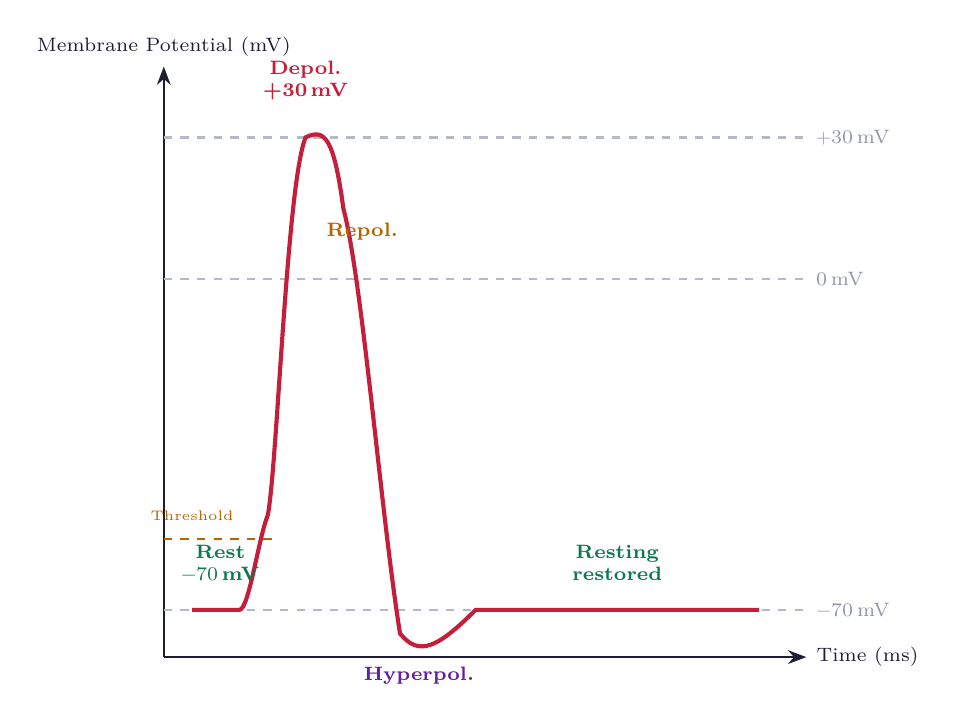
\begin{tikzpicture}[x=1.2cm, y=0.060cm, thick]
  % Axes
  \draw[arrow] (-0.3, -80) -- (6.5, -80) node[right, font=\scriptsize] {Time (ms)};
  \draw[arrow] (-0.3, -80) -- (-0.3, 45) node[above, font=\scriptsize] {Membrane Potential (mV)};

  % Resting potential line
  \draw[dashed, color=mgframe] (-0.3, -70) -- (6.5, -70) node[right, font=\scriptsize, color=watermark] {$-70\,\text{mV}$};
  \draw[dashed, color=mgframe] (-0.3, 0) -- (6.5, 0) node[right, font=\scriptsize, color=watermark] {$0\,\text{mV}$};
  \draw[dashed, color=mgframe] (-0.3, 30) -- (6.5, 30) node[right, font=\scriptsize, color=watermark] {$+30\,\text{mV}$};

  % Waveform
  \draw[color=myred, line width=1.5pt]
    (0.0, -70) -- (0.5, -70)
    .. controls (0.6, -70) and (0.7, -55) .. (0.8, -50)
    .. controls (0.9, -40) and (1.0, 20) .. (1.2, 30)
    .. controls (1.4, 32) and (1.5, 30) .. (1.6, 15)
    .. controls (1.8, 0) and (2.0, -50) .. (2.2, -75)
    .. controls (2.4, -80) and (2.6, -78) .. (3.0, -70)
    -- (6.0, -70);

  % Phase labels
  \node[font=\scriptsize\bfseries, color=mygreen, align=center] at (0.3, -60) {Rest\\\scriptsize $-70$\,mV};
  \node[font=\scriptsize\bfseries, color=myred, align=center] at (1.2, 42) {Depol.\\+30\,mV};
  \node[font=\scriptsize\bfseries, color=myamber, align=center] at (1.8, 10) {Repol.};
  \node[font=\scriptsize\bfseries, color=mypurple, align=center] at (2.4, -84) {Hyperpol.};
  \node[font=\scriptsize\bfseries, color=mygreen, align=center] at (4.5, -60) {Resting\\restored};

  % Threshold marker
  \draw[dashed, color=myamber, thin] (-0.3, -55) -- (0.85, -55);
  \node[font=\tiny, color=myamber] at (0.0, -50) {Threshold};
\end{tikzpicture}
\end{tcolorbox}

\subsection{The Brain and EEG Signals}

The brain generates rhythmic electrical activity that can be recorded as an \textbf{Electroencephalogram (EEG)} from scalp electrodes. Different frequency bands correspond to different states of consciousness:

\par\noindent
\begin{tabularx}{\linewidth}{|B{2.2cm}|>{\centering\arraybackslash}m{2.2cm}|>{\centering\arraybackslash}m{2.2cm}|Y|}
\hline
\textbf{Wave} & \textbf{\color{myteal}Freq. (Hz)} & \textbf{\color{myamber}Amplitude ($\mu$V)} & \textbf{State} \\
\hline
\textbf{Delta ($\delta$)} & 0.5 -- 4 & 20 -- 200 & Deep sleep (slow-wave sleep). \\
\hline
\textbf{Theta ($\theta$)} & 4 -- 8 & 20 -- 100 & Drowsiness, light sleep, creativity. \\
\hline
\textbf{Alpha ($\alpha$)} & 8 -- 13 & 20 -- 60 & Relaxed wakefulness, eyes closed. \\
\hline
\textbf{Beta ($\beta$)} & 13 -- 30 & 5 -- 30 & Active thinking, concentration, alert. \\
\hline
\textbf{Gamma ($\gamma$)} & 30 -- 100 & $< 10$ & Intense cognitive processing. \\
\hline
\end{tabularx}

% ===============================================================================
\section{The Muscular System and Bio-Electrical Signals Summary}
% ===============================================================================

\begin{tcolorbox}[defbox, title={\textbf{Types of Muscle Tissue}}]
\begin{itemize}[leftmargin=*, itemsep=2.5pt, topsep=0pt]
  \item \textbf{Skeletal Muscle:} Voluntary, striated, attached to bones. Controlled by the somatic nervous system. Generates \textbf{EMG} signals.
  \item \textbf{Cardiac Muscle:} Involuntary, striated, forms the heart wall. Self-excitable via SA node. Generates \textbf{ECG} signals.
  \item \textbf{Smooth Muscle:} Involuntary, non-striated, found in blood vessel walls, digestive tract, lungs. Controlled by the autonomic nervous system.
\end{itemize}
\end{tcolorbox}

\subsection{Summary of Bio-Electrical Signals}

\par\noindent
\begin{tabularx}{\linewidth}{|B{2.0cm}|Y|>{\centering\arraybackslash}m{2.2cm}|>{\centering\arraybackslash}m{2.6cm}|}
\hline
\textbf{Signal} & \textbf{\color{myteal}Physiological Origin} & \textbf{\color{myamber}Amplitude} & \textbf{\color{mygreen}Frequency Range} \\
\hline
\textbf{ECG} & Cardiac muscle depolarization/repolarization. & 0.5 -- 4 mV & 0.05 -- 150 Hz \\
\hline
\textbf{EMG} & Skeletal muscle fibre action potentials (motor units). & 0.1 -- 5 mV & 5 -- 2000 Hz \\
\hline
\textbf{EEG} & Aggregate cortical neuron activity (brain). & 5 -- 300 $\mu$V & 0.5 -- 100 Hz \\
\hline
\textbf{EOG} & Retinal dipole movement with eye motion. & 0.5 -- 1 mV & DC -- 100 Hz \\
\hline
\textbf{ERG} & Retinal response to light stimulation. & 0.5 -- 1 mV & DC -- 50 Hz \\
\hline
\textbf{EGG} & Gastro-intestinal smooth muscle electrical activity. & 0.1 -- 1 mV & 0.05 -- 1 Hz \\
\hline
\end{tabularx}

\newpage
% ===============================================================================
% MANDATORY QUICK REVISION PAGE
% ===============================================================================
\begin{center}
  {\large\bfseries\color{myred} Quick Revision --- Module 1}\\[3pt]
  {\small\color{mydark} Introduction to Human Physiology $|$ PE-EC603B}
\end{center}
\noindent{\color{myred}\rule{\linewidth}{1.2pt}}
\vspace{4pt}

\begin{tcolorbox}[formulabox, title={\textbf{Key Formulas and Normal Values}}]
\renewcommand{\arraystretch}{1.3}
\begin{tabularx}{\linewidth}{B{4.0cm} X}
Cardiac Output & $CO = HR \times SV$ \quad ($\approx 5\,\text{L/min}$ at rest) \\[4pt]
Mean Arterial Pressure & $MAP = \displaystyle\frac{SBP + 2\times DBP}{3}$ \\[8pt]
Total Lung Capacity & $TLC = TV + IRV + ERV + RV \approx 5800\,\text{mL}$ \\[4pt]
Vital Capacity & $VC = TV + IRV + ERV \approx 4600\,\text{mL}$ \\[4pt]
Nernst Equation (ion potential) & $E = \displaystyle\frac{RT}{zF}\ln\frac{[\text{ion}]_{\text{out}}}{[\text{ion}]_{\text{in}}}$ \\[8pt]
Resting Membrane Potential & $\approx -70\,\text{mV}$ (inside negative)
\end{tabularx}
\end{tcolorbox}

\begin{tcolorbox}[defbox, title={\textbf{One-Line Definitions}}]
\begin{itemize}[leftmargin=*, itemsep=2.5pt, topsep=0pt]
  \item \textbf{Homeostasis:} The body's ability to maintain a stable internal environment via negative feedback loops.
  \item \textbf{SA Node:} Sinoatrial node; the heart's natural pacemaker located in the right atrium; fires at $60$--$100\,\text{bpm}$.
  \item \textbf{Action Potential:} A brief, self-propagating reversal of membrane polarity ($-70$ to $+30\,\text{mV}$) that transmits nerve signals.
  \item \textbf{Cardiac Output:} Volume of blood pumped per minute by either ventricle; $CO = HR \times SV$.
  \item \textbf{Tidal Volume:} Volume of air inhaled or exhaled in one normal, quiet breath ($\approx 500\,\text{mL}$).
  \item \textbf{Vital Capacity:} Maximum volume of air a person can expire after a maximal inspiration.
  \item \textbf{Depolarization:} Rapid influx of $\text{Na}^+$ ions causing the cell membrane to become positive inside.
  \item \textbf{ECG:} Electrocardiogram; surface recording of the heart's electrical activity.
  \item \textbf{EEG:} Electroencephalogram; scalp recording of brain electrical activity.
  \item \textbf{EMG:} Electromyogram; recording of skeletal muscle electrical activity.
\end{itemize}
\end{tcolorbox}

\begin{tcolorbox}[exambox, title={\textbf{Frequently Asked / Viva Questions}}]
\begin{enumerate}[topsep=0pt, label=\textbf{Q\arabic*.}, itemsep=5pt]
  \item \Q{What is homeostasis? Give an example.}
    Homeostasis is the maintenance of a stable internal environment through negative feedback. Example: If body temperature rises, sweat glands are activated to cool the body back to $37\,^{\circ}\text{C}$.
  \item \Q{Describe the role of the SA node in the heart.}
    The SA node is the natural cardiac pacemaker located in the right atrium. It spontaneously depolarizes at $60$--$100\,\text{bpm}$, initiating an electrical impulse that propagates to the AV node, bundle of His, and Purkinje fibres, triggering coordinated ventricular contraction.
  \item \Q{What physiological event does the QRS complex of the ECG represent?}
    The QRS complex represents ventricular depolarization --- the electrical event that triggers the simultaneous contraction of the left and right ventricles.
  \item \Q{Define cardiac output and state its normal value.}
    Cardiac Output (CO) is the volume of blood ejected by one ventricle per minute: $CO = HR \times SV \approx 5\,\text{L/min}$ at rest for an adult.
  \item \Q{What is the difference between systolic and diastolic blood pressure?}
    Systolic pressure ($\approx 120\,\text{mmHg}$) is the peak pressure in the arteries during ventricular contraction. Diastolic pressure ($\approx 80\,\text{mmHg}$) is the minimum pressure during ventricular relaxation.
  \item \Q{Explain the all-or-nothing law of nerve conduction.}
    Once a stimulus exceeds the threshold (about $-55\,\text{mV}$), a full action potential of fixed amplitude is triggered. A sub-threshold stimulus produces no action potential at all. The amplitude does not increase with stronger stimuli.
  \item \Q{List the EEG wave bands and their corresponding brain states.}
    Delta ($0.5$--$4\,\text{Hz}$): deep sleep; Theta ($4$--$8\,\text{Hz}$): drowsiness; Alpha ($8$--$13\,\text{Hz}$): relaxed wakefulness; Beta ($13$--$30\,\text{Hz}$): active alertness; Gamma ($>30\,\text{Hz}$): intense cognition.
  \item \Q{What is the difference between ECG, EMG, and EEG signals in terms of amplitude and frequency?}
    ECG: $0.5$--$4\,\text{mV}$, $0.05$--$150\,\text{Hz}$ (cardiac). EMG: $0.1$--$5\,\text{mV}$, $5$--$2000\,\text{Hz}$ (skeletal muscle). EEG: $5$--$300\,\mu\text{V}$, $0.5$--$100\,\text{Hz}$ (brain) --- much smaller amplitude than ECG or EMG.
  \item \Q{What is the role of the myelin sheath in nerve conduction?}
    The myelin sheath acts as an electrical insulator around the axon. Depolarization jumps between nodes of Ranvier (saltatory conduction), dramatically increasing conduction velocity to $40$--$70\,\text{m/s}$ compared to $0.5$--$2\,\text{m/s}$ in unmyelinated fibres.
  \item \Q{Define tidal volume and vital capacity.}
    Tidal Volume (TV) is the volume of air inhaled/exhaled per normal breath ($\approx 500\,\text{mL}$). Vital Capacity (VC) is the maximum air that can be expelled after maximum inhalation ($VC = TV + IRV + ERV \approx 4600\,\text{mL}$).
  \item \Q{Why is the left ventricular wall thicker than the right?}
    The left ventricle pumps blood through the systemic circulation (entire body), working against a much higher resistance (pressure $\approx 120\,\text{mmHg}$). The right ventricle only pumps to the lungs (pulmonary pressure $\approx 25\,\text{mmHg}$), so it needs less force.
\end{enumerate}
\end{tcolorbox}

\begin{tcolorbox}[tikzbox, title={Bio-Electrical Signal Comparison}]
\renewcommand{\arraystretch}{1.4}
\par\noindent
\begin{tabularx}{\linewidth}{|B{1.8cm}|>{\small\centering\arraybackslash}X|>{\small\centering\arraybackslash}X|>{\small\centering\arraybackslash}X|}
\hline
\textbf{Signal} & \textbf{\color{myred}ECG} & \textbf{\color{myteal}EMG} & \textbf{\color{mypurple}EEG} \\
\hline
Source & Heart muscle & Skeletal muscle & Brain cortex \\
\hline
Amplitude & 0.5 -- 4 mV & 0.1 -- 5 mV & 5 -- 300 $\mu$V \\
\hline
Bandwidth & 0.05 -- 150 Hz & 5 -- 2000 Hz & 0.5 -- 100 Hz \\
\hline
Electrodes & Surface, chest & Surface/needle & Scalp (10-20 system) \\
\hline
Clinical use & Arrhythmia, ischemia & Neuropathy, NCV & Epilepsy, sleep disorders \\
\hline
\end{tabularx}
\end{tcolorbox}


% -- Module 2 -----------------------------------------------------------------
\modulestart{2}{Biomedical Transducers --- Classification and Characteristics}

\section{Biomedical Transducers --- Classification and Characteristics}
% ===============================================================================

\begin{tcolorbox}[defbox, title={\textbf{Definition: Biomedical Transducer}}]
A \textbf{biomedical transducer} is a device that converts a physiological (biological or physical) variable into an electrical signal suitable for measurement, display, recording, or processing. It acts as the primary sensing element in a medical instrument.
\end{tcolorbox}

\subsection{Classification of Biomedical Transducers}

\textbf{1. By Transduction Principle:}\par\noindent
\begin{tabularx}{\linewidth}{|B{3.0cm}|Y|Y|}
\hline
\textbf{Type} & \textbf{\color{myteal}Principle} & \textbf{\color{mygreen}Example} \\
\hline
\textbf{Resistive} & Measured quantity changes resistance. & Strain gauge, thermistor, potentiometer. \\
\hline
\textbf{Capacitive} & Measured quantity changes capacitance. & Capacitive pressure sensor, microphone. \\
\hline
\textbf{Inductive / LVDT} & Movement changes mutual inductance. & LVDT (Linear Variable Differential Transformer). \\
\hline
\textbf{Piezoelectric} & Mechanical stress produces a voltage. & Ultrasonic transducer, force sensor. \\
\hline
\textbf{Photoelectric} & Light intensity changes output current. & Pulse oximeter, photodiode sensor. \\
\hline
\textbf{Electrochemical} & Ion concentration generates EMF. & pH electrode, ion-selective electrode. \\
\hline
\textbf{Thermoelectric} & Temperature difference generates voltage. & Thermocouple (Seebeck effect). \\
\hline
\end{tabularx}

\textbf{2. By Input Quantity:} Displacement, Velocity, Force, Pressure, Acceleration, Flow, Temperature, Potential, Chemical concentration.

\subsection{Desirable Characteristics of a Biomedical Transducer}

\begin{itemize}[leftmargin=*, itemsep=3pt]
  \item \textbf{High Sensitivity:} Large output per unit physiological change.
  \item \textbf{High Linearity:} Output proportional to input over the full range.
  \item \textbf{Low Hysteresis:} Output should not depend on direction of change.
  \item \textbf{High Signal-to-Noise Ratio (SNR):} Minimum interference and noise pick-up.
  \item \textbf{Biocompatibility:} Non-toxic, non-irritating, and chemically inert when implanted or in contact with tissue.
  \item \textbf{Minimal Loading Effect:} The transducer should not disturb the physiological system it is measuring.
  \item \textbf{Stability and Reproducibility:} Consistent readings over time and repeated measurements.
\end{itemize}

% ===============================================================================
\section{Displacement and Velocity Transducers}
% ===============================================================================

\subsection{Strain Gauge (Resistive)}

\begin{tcolorbox}[defbox, title={\textbf{Strain Gauge}}]
A \textbf{strain gauge} is a resistive sensor whose electrical resistance changes proportionally to the mechanical strain (deformation) applied to it. Used to measure force, pressure, torque, and displacement indirectly.
\end{tcolorbox}

\begin{tcolorbox}[formulabox, title={\textbf{Strain Gauge Formula}}]
\[
\frac{\Delta R}{R} = G_F \cdot \varepsilon
\]
where $\varepsilon = \dfrac{\Delta L}{L}$ is the mechanical strain, and $G_F$ is the \textbf{Gauge Factor} (typically $2$ for metal foil gauges; up to $150$ for semiconductor gauges).
\[
G_F = \frac{\Delta R/R}{\varepsilon} = 1 + 2\nu + \pi_\ell E
\]
$\nu$ = Poisson's ratio; $\pi_\ell$ = piezoresistive coefficient; $E$ = Young's modulus.
\end{tcolorbox}

Strain gauges are arranged in a \textbf{Wheatstone bridge} to improve sensitivity and temperature compensation. For blood pressure measurement, the strain gauge is bonded to a stainless steel diaphragm.

\subsection{LVDT (Linear Variable Differential Transformer)}

\begin{tcolorbox}[defbox, title={\textbf{LVDT}}]
The \textbf{Linear Variable Differential Transformer (LVDT)} is an inductive displacement sensor that produces an AC voltage output proportional to the linear displacement of a movable ferromagnetic core.
\end{tcolorbox}

\begin{tcolorbox}[tikzbox, title={LVDT Schematic Diagram}]
\centering
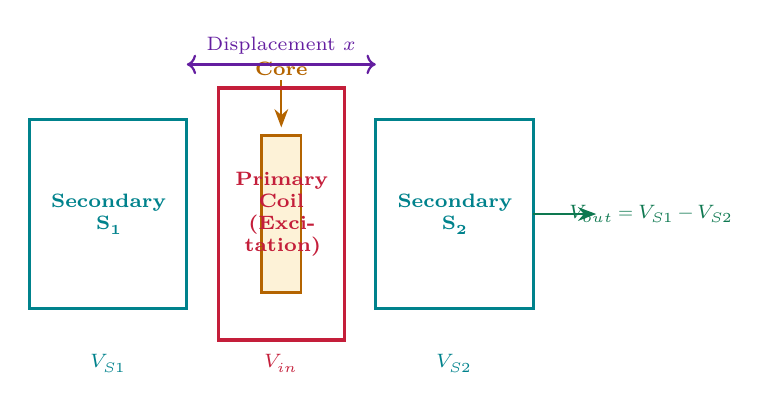
\begin{tikzpicture}[thick, font=\small]
  % Core (movable)
  \filldraw[fill=hdramber, draw=myamber, line width=1pt] (0.55, 0.6) rectangle (1.05, 2.6);
  \node[color=myamber, font=\scriptsize\bfseries] at (0.8, 3.45) {Core};
  \draw[arrow, color=myamber] (0.8, 3.3) -- (0.8, 2.7);

  % Primary coil (centre)
  \draw[color=myred, line width=1.2pt] (0, 0) rectangle (1.6, 3.2);
  \node[color=myred, font=\scriptsize\bfseries, align=center, text width=1.5cm] at (0.8, 1.6) {Primary\\Coil\\(Excitation)};

  % Secondary coil S1 (left)
  \draw[color=myteal, line width=1.2pt] (-2.4, 0.4) rectangle (-0.4, 2.8);
  \node[color=myteal, font=\scriptsize\bfseries, align=center, text width=1.5cm] at (-1.4, 1.6) {Secondary\\S\textsubscript{1}};

  % Secondary coil S2 (right)
  \draw[color=myteal, line width=1.2pt] (2.0, 0.4) rectangle (4.0, 2.8);
  \node[color=myteal, font=\scriptsize\bfseries, align=center, text width=1.5cm] at (3.0, 1.6) {Secondary\\S\textsubscript{2}};

  % Displacement arrow
  \draw[<->, color=mypurple, thick] (-0.4, 3.5) -- (2.0, 3.5) node[midway, above, font=\scriptsize, color=mypurple] {Displacement $x$};

  % Output labels
  \node[font=\scriptsize, color=myteal] at (-1.4, -0.3) {$V_{S1}$};
  \node[font=\scriptsize, color=myteal] at (3.0, -0.3) {$V_{S2}$};
  \node[font=\scriptsize, color=myred] at (0.8, -0.3) {$V_{in}$};
  \node[font=\scriptsize, color=mygreen] at (5.5, 1.6) {$V_{out} = V_{S1} - V_{S2}$};
  \draw[arrow, color=mygreen] (4.0, 1.6) -- (4.8, 1.6);
\end{tikzpicture}
\end{tcolorbox}

\textbf{Working:} When the core is at the centre (null position), $V_{S1} = V_{S2}$, so $V_{out} = 0$. Displacement to one side increases coupling to that secondary coil, creating a differential output proportional to displacement. The output phase indicates direction of displacement.

\textbf{Biomedical Applications:} Measuring chest wall movement during respiration, arterial diameter pulsation, bone growth measurement.

% ===============================================================================
\section{Force, Pressure, and Acceleration Transducers}
% ===============================================================================

\subsection{Piezoelectric Transducer}

\begin{tcolorbox}[defbox, title={\textbf{Piezoelectric Effect}}]
The \textbf{piezoelectric effect} is the generation of an electric charge on certain crystalline materials (e.g., quartz, PZT --- Lead Zirconate Titanate, PVDF) when they are subjected to mechanical stress or deformation. Conversely, an applied electric field causes the material to deform (\textbf{converse piezoelectric effect}).
\end{tcolorbox}

\begin{tcolorbox}[formulabox, title={\textbf{Piezoelectric Sensor Equations}}]
\[
Q = d_{ij} \cdot F \qquad V_{out} = \frac{Q}{C_p} = \frac{d_{ij} \cdot F}{C_p}
\]
where $Q$ = generated charge (C), $d_{ij}$ = piezoelectric charge constant (C/N), $F$ = applied force (N), $C_p$ = sensor capacitance (F). \\[4pt]
Sensitivity: $S = \dfrac{V_{out}}{F} = \dfrac{d_{ij}}{C_p}$ \quad (V/N)
\end{tcolorbox}

\textbf{Biomedical Applications:} Ultrasonic imaging transducers (transmit and receive), phonocardiography (heart sound recording), pulse waveform measurement, bone conduction hearing aids.

\textbf{Limitations:} Cannot measure static forces (DC signals bleed away through parasitic resistance). Requires high-input-impedance amplifiers.

\subsection{Capacitive Pressure Sensor}

A capacitive pressure sensor uses a flexible diaphragm as one plate of a capacitor. Applied pressure deflects the diaphragm, changing the gap $d$:
\[
C = \frac{\varepsilon_0 \varepsilon_r A}{d} \qquad \Rightarrow \qquad \Delta C \propto \Delta P
\]
Used in blood pressure catheters, intra-cranial pressure (ICP) monitoring.

\subsection{Accelerometer}

\begin{tcolorbox}[defbox, title={\textbf{Accelerometer}}]
An \textbf{accelerometer} is a transducer that measures acceleration (rate of change of velocity), typically based on a proof mass attached to a spring-damper system. Used to assess patient movement, gait analysis, and in implantable cardiac pacemakers (rate-responsive pacing).
\end{tcolorbox}

$F = ma \Rightarrow$ deflection of mass proportional to acceleration. Piezoresistive or capacitive sensing of the deflection gives output voltage $\propto$ acceleration.

% ===============================================================================
\section{Flow and Temperature Transducers}
% ===============================================================================

\subsection{Electromagnetic Blood Flow Transducer}

\begin{tcolorbox}[defbox, title={\textbf{Electromagnetic Flowmeter}}]
Based on \textbf{Faraday's law of electromagnetic induction}: when a conductor (blood, which contains ions) moves through a magnetic field, an EMF is induced perpendicular to both the flow direction and the magnetic field.
\end{tcolorbox}

\begin{tcolorbox}[formulabox, title={\textbf{Electromagnetic Flowmeter Formula}}]
\[
V_{emf} = B \cdot d \cdot v
\]
where $B$ = magnetic flux density (T), $d$ = inner diameter of vessel (m), $v$ = mean blood velocity (m/s). \\[4pt]
Volumetric Flow Rate: $Q = v \cdot A = v \cdot \dfrac{\pi d^2}{4}$
\end{tcolorbox}

\textbf{Advantages:} No obstruction to flow, direct velocity measurement, works with pulsatile flow. \textbf{Limitation:} Requires surgical placement around the vessel (perivascular cuff type).

\subsection{Ultrasonic (Doppler) Flow Transducer}

When ultrasound is transmitted into blood and reflected from moving red blood cells, the reflected frequency is shifted:
\[
\Delta f = f_r - f_t = \frac{2 f_t \cdot v \cdot \cos\theta}{c}
\]
where $v$ = blood velocity, $\theta$ = angle between ultrasound beam and flow direction, $c$ = speed of sound in tissue ($\approx 1540\,\text{m/s}$). \\[4pt]
Non-invasive, used in vascular Doppler studies and echocardiography.

\subsection{Temperature Transducers}

\par\noindent
\begin{tabularx}{\linewidth}{|B{2.8cm}|Y|>{\centering\arraybackslash}m{2.0cm}|Y|}
\hline
\textbf{Type} & \textbf{\color{myteal}Principle} & \textbf{\color{myamber}Range} & \textbf{\color{mygreen}Biomedical Use} \\
\hline
\textbf{Thermistor} & NTC/PTC semiconductor resistance vs.\ temperature. & $-50$ to $150\,^{\circ}$C & Rectal/skin/blood temp. \\
\hline
\textbf{Thermocouple} & Seebeck effect: voltage at junction of dissimilar metals. & $-200$ to $1200\,^{\circ}$C & Surgical probes, cryosurgery. \\
\hline
\textbf{RTD (Pt100)} & Platinum resistance increases linearly with temperature. & $-200$ to $600\,^{\circ}$C & Precision lab instruments. \\
\hline
\textbf{IC Sensor} & Semiconductor bandgap vs.\ temperature (e.g., LM35). & $-55$ to $150\,^{\circ}$C & Clinical thermometers. \\
\hline
\end{tabularx}

\textbf{Thermistor Equation (NTC):}
\[
R_T = R_0 \cdot e^{B\left(\frac{1}{T} - \frac{1}{T_0}\right)}
\]
where $B$ = material constant ($2000$--$5000\,\text{K}$), $T$ = temperature in Kelvin, $R_0$ = resistance at reference temperature $T_0$.

% ===============================================================================
\section{Chemical and Ion-Selective Transducers}
% ===============================================================================

\begin{tcolorbox}[defbox, title={\textbf{Ion-Selective Electrode (ISE)}}]
An \textbf{ion-selective electrode} generates a potential proportional to the logarithm of the concentration of a specific ion (e.g., $\text{Na}^+$, $\text{K}^+$, $\text{Ca}^{2+}$, $\text{H}^+$) in the solution according to the \textbf{Nernst equation}.
\end{tcolorbox}

\begin{tcolorbox}[formulabox, title={\textbf{Nernst Equation and pH Electrode}}]
\[
E = E^0 + \frac{RT}{zF}\ln[\text{ion}] \quad = E^0 - \frac{0.0592}{z}\log[\text{ion}] \quad \text{(at } 25\,^{\circ}\text{C)}
\]
For \textbf{pH electrode} ($z=1$ for H\textsuperscript{+}): $E = E^0 - 59.2\,\text{mV} \times \text{pH}$ \quad (Sensitivity: $59.2\,\text{mV/pH}$)
\end{tcolorbox}

\textbf{Dissolved Gas Sensors:}
\begin{itemize}[leftmargin=*, itemsep=3pt]
  \item \textbf{Clark Electrode (pO\textsubscript{2}):} Amperometric sensor. O\textsubscript{2} is reduced at a platinum cathode through a semipermeable membrane; current is proportional to $\text{pO}_2$.
  \item \textbf{Severinghaus Electrode (pCO\textsubscript{2}):} CO\textsubscript{2} diffuses through a membrane into bicarbonate solution, changing its pH, measured by a pH electrode.
\end{itemize}

% ===============================================================================
\section{Bio-electrodes}
% ===============================================================================

\begin{tcolorbox}[defbox, title={\textbf{Bio-electrode}}]
A \textbf{bio-electrode} is an interface between the biological medium (ionic conduction) and the measurement circuitry (electronic conduction). It converts ionic current flow in tissues to electron current flow in metallic wires.
\end{tcolorbox}

\subsection{Electrode--Electrolyte Interface and Half-Cell Potential}

At the electrode--electrolyte interface, oxidation/reduction reactions create a \textbf{half-cell potential} $E_{HC}$. For a metal electrode:
\[
M \rightleftharpoons M^{n+} + ne^- \qquad E_{HC} = E^0 + \frac{RT}{nF}\ln[M^{n+}]
\]
The \textbf{electrode offset potential} creates a DC bias that can saturate amplifiers if not accounted for.

\subsection{Types of Electrodes}

\par\noindent
\begin{tabularx}{\linewidth}{|B{2.8cm}|Y|Y|}
\hline
\textbf{Type} & \textbf{\color{myteal}Description} & \textbf{\color{mygreen}Application} \\
\hline
\textbf{Ag/AgCl Surface} & Silver coated with AgCl paste; very stable, low offset potential. & Standard ECG chest electrodes, EEG. \\
\hline
\textbf{Carbon / Paste} & Conductive carbon paste; disposable, low cost. & Holter monitor, disposable ECG patches. \\
\hline
\textbf{Needle Electrode} & Fine steel or platinum needle inserted into muscle. & Clinical EMG recording, nerve conduction. \\
\hline
\textbf{Concentric Needle} & Inner wire in insulated cannula; records single motor unit. & Single motor unit EMG. \\
\hline
\textbf{Floating Electrode} & Electrode body floats; electrolyte gel bridges skin. & Long-term ambulatory monitoring. \\
\hline
\textbf{Suction Electrode} & Adheres to skin via suction (no adhesive). & Chest ECG, temporary use. \\
\hline
\textbf{Microelectrode} & Glass capillary filled with KCl; tip $< 1\,\mu\text{m}$. & Intracellular recording of action potentials. \\
\hline
\end{tabularx}

\textbf{Equivalent circuit of a bio-electrode:} Series combination of half-cell potential $E_{HC}$, electrode resistance $R_e$, and double-layer capacitance $C_d$, in series with the tissue resistance $R_t$.

% ===============================================================================
\section{Bio-potential Amplifiers and Signals}
% ===============================================================================

\subsection{Requirements of a Bio-potential Amplifier}

Bio-electrical signals (ECG, EMG, EEG) have very small amplitudes ($\mu$V to mV range) contaminated by electrode offset potentials, motion artefacts, and 50/60 Hz power-line interference. A bio-potential amplifier must have:

\begin{itemize}[leftmargin=*, itemsep=3pt]
  \item \textbf{Very High Input Impedance} ($> 10\,\text{M}\Omega$): To minimize loading of the high-impedance electrode--skin interface.
  \item \textbf{High Common Mode Rejection Ratio (CMRR)} ($> 80\,\text{dB}$): To reject the 50 Hz power-line interference which appears as a common-mode signal on both input electrodes.
  \item \textbf{Low Noise:} Input-referred noise $< 1\,\mu\text{V}_{rms}$ for EEG.
  \item \textbf{High Gain:} Sufficient to bring signals to ADC-compatible levels (typically $\times 1000$).
  \item \textbf{Appropriate Bandwidth:} ECG: $0.05$--$150\,\text{Hz}$; EMG: $5$--$2000\,\text{Hz}$; EEG: $0.5$--$100\,\text{Hz}$.
  \item \textbf{Patient Safety Isolation:} Galvanic isolation (optocouplers or transformers) to prevent micro-shock from leakage currents.
\end{itemize}

\subsection{Instrumentation Amplifier (INA)}

The \textbf{instrumentation amplifier (INA)} is the standard front-end for bio-potential amplifiers. It consists of three op-amps:

\begin{tcolorbox}[tikzbox, title={3-Op-Amp Instrumentation Amplifier Block Diagram}]
\centering
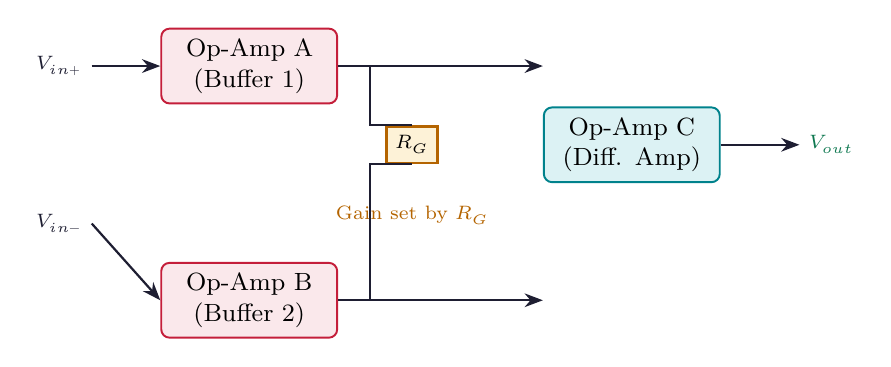
\begin{tikzpicture}[node distance=1.2cm and 2.2cm, thick, font=\small]
  % Input buffer op-amps
  \node[redblock, text width=2.0cm] (opA) {Op-Amp A\\(Buffer 1)};
  \node[redblock, text width=2.0cm, below=2.0cm of opA] (opB) {Op-Amp B\\(Buffer 2)};
  \node[block, text width=2.0cm, right=2.6cm of opA, yshift=-1.0cm] (opC) {Op-Amp C\\(Diff. Amp)};

  % Resistor Rg
  \node[draw=myamber, fill=hdramber, minimum width=0.6cm, minimum height=0.35cm,
        font=\scriptsize, right=0.6cm of opA, yshift=-1.0cm] (Rg) {$R_G$};

  % Input labels
  \draw[arrow] (-2.0, 0) node[left, font=\scriptsize] {$V_{in+}$} -- (opA.west);
  \draw[arrow] (-2.0, -2.0) node[left, font=\scriptsize] {$V_{in-}$} -- (opB.west);

  % Connect buffers to Rg
  \draw[line] (opA.east) -- ++(0.4,0) |- (Rg.north);
  \draw[line] (opB.east) -- ++(0.4,0) |- (Rg.south);

  % Connect buffers to diff amp
  \draw[arrow] (opA.east) -- ++(0.4,0) -- ++(0.9,0) |- (opC.west |- opA);
  \draw[arrow] (opB.east) -- ++(0.4,0) -- ++(0.9,0) |- (opC.west |- opB);

  % Output
  \draw[arrow] (opC.east) -- ++(1.0, 0) node[right, font=\scriptsize, color=mygreen] {$V_{out}$};

  % Gain label
  \node[font=\scriptsize, color=myamber, below=0.4cm of Rg] {Gain set by $R_G$};
\end{tikzpicture}
\end{tcolorbox}

\begin{tcolorbox}[formulabox, title={\textbf{Instrumentation Amplifier Gain Formula}}]
\[
A_V = \left(1 + \frac{2R}{R_G}\right) \cdot \frac{R_f}{R_1}
\]
where $R_G$ is the single external gain-setting resistor. Increasing $R_G$ decreases gain; $R_G \to \infty$ gives $A_V \to 1$ (unity gain). \\[4pt]
\textbf{CMRR (dB)} $= 20\log_{10}\left(\frac{A_{dm}}{A_{cm}}\right)$ \quad Typical: $80$--$120\,\text{dB}$ for medical-grade amplifiers.
\end{tcolorbox}

\subsection{ECG, EMG, and EEG Amplifier Comparison}

\par\noindent
\begin{tabularx}{\linewidth}{|B{2.0cm}|>{\centering\arraybackslash}m{2.0cm}|>{\centering\arraybackslash}m{2.3cm}|>{\centering\arraybackslash}m{2.0cm}|Y|}
\hline
\textbf{Signal} & \textbf{\color{myteal}Amplitude} & \textbf{\color{myamber}Bandwidth} & \textbf{\color{myred}Gain} & \textbf{Key Considerations} \\
\hline
\textbf{ECG} & 0.5--4 mV & 0.05--150 Hz & 1000 & High CMRR for 50 Hz rejection; right-leg drive circuit. \\
\hline
\textbf{EMG} & 0.1--5 mV & 5--2000 Hz & 500--5000 & Wide bandwidth; needle or surface electrodes. \\
\hline
\textbf{EEG} & 5--300 $\mu$V & 0.5--100 Hz & 10\,000--100\,000 & Extremely low noise; 19+ channel 10-20 system. \\
\hline
\end{tabularx}

\newpage
% ===============================================================================
% MANDATORY QUICK REVISION PAGE
% ===============================================================================
\begin{center}
  {\large\bfseries\color{myred} Quick Revision --- Module 2}\\[3pt]
  {\small\color{mydark} Biomedical Transducers and Bio-potential Amplifiers $|$ PE-EC603B}
\end{center}
\noindent{\color{myred}\rule{\linewidth}{1.2pt}}
\vspace{4pt}

\begin{tcolorbox}[formulabox, title={\textbf{Key Formulas}}]
\renewcommand{\arraystretch}{1.3}
\begin{tabularx}{\linewidth}{B{4.2cm} X}
Strain Gauge Sensitivity & $\dfrac{\Delta R}{R} = G_F \cdot \varepsilon$; \quad $G_F \approx 2$ (metal), $\approx 100$ (semiconductor). \\[8pt]
Piezoelectric Voltage & $V_{out} = \dfrac{d_{ij} \cdot F}{C_p}$ \\[8pt]
Thermistor (NTC) & $R_T = R_0 \cdot e^{B(1/T - 1/T_0)}$ \\[4pt]
Nernst / pH & $E = E^0 - 59.2 \times \text{pH}\ \text{mV}$ at $25\,^{\circ}\text{C}$ \\[4pt]
EM Flowmeter & $V_{emf} = B \cdot d \cdot v$ \\[4pt]
Doppler Shift & $\Delta f = \dfrac{2 f_t v \cos\theta}{c}$ \\[8pt]
INA Gain & $A_V = \left(1 + \dfrac{2R}{R_G}\right)\dfrac{R_f}{R_1}$ \\[8pt]
CMRR & $CMRR\,(dB) = 20\log_{10}(A_{dm}/A_{cm})$
\end{tabularx}
\end{tcolorbox}

\begin{tcolorbox}[defbox, title={\textbf{One-Line Definitions}}]
\begin{itemize}[leftmargin=*, itemsep=2.5pt, topsep=0pt]
  \item \textbf{Transducer:} Device converting a physiological variable into an electrical signal.
  \item \textbf{Gauge Factor ($G_F$):} Ratio of relative change in resistance to applied strain.
  \item \textbf{LVDT:} Inductive displacement transducer whose output voltage is proportional to core displacement.
  \item \textbf{Piezoelectric Effect:} Generation of charge under mechanical stress in crystals like quartz or PZT.
  \item \textbf{Thermistor:} Semiconductor temperature sensor with a large negative (NTC) or positive (PTC) temperature coefficient of resistance.
  \item \textbf{Ag/AgCl Electrode:} The standard body surface bio-electrode; stable half-cell potential, low offset drift.
  \item \textbf{Half-cell Potential:} DC potential at the electrode-electrolyte interface due to ion exchange reactions.
  \item \textbf{CMRR:} Common Mode Rejection Ratio; ability of an amplifier to reject signals common to both input terminals (e.g., 50 Hz noise).
  \item \textbf{Instrumentation Amplifier:} Three-op-amp differential amplifier with high input impedance and high CMRR used for bio-signal acquisition.
  \item \textbf{Clark Electrode:} Amperometric sensor measuring dissolved oxygen partial pressure ($\text{pO}_2$).
\end{itemize}
\end{tcolorbox}

\begin{tcolorbox}[exambox, title={\textbf{Frequently Asked / Viva Questions}}]
\begin{enumerate}[topsep=0pt, label=\textbf{Q\arabic*.}, itemsep=5pt]
  \item \Q{Define gauge factor. What is its typical value for metal and semiconductor strain gauges?}
    Gauge factor $G_F = (\Delta R / R) / \varepsilon$. For metal foil gauges, $G_F \approx 2$. For semiconductor (silicon) gauges, $G_F \approx 100$--$150$, offering much higher sensitivity.
  \item \Q{Explain the working principle of an LVDT.}
    An AC voltage excites the primary coil. The ferromagnetic core couples this flux to two secondary coils differentially. Displacement of the core increases coupling to one secondary and decreases it to the other, producing an output voltage ($V_{S1} - V_{S2}$) proportional to the displacement. Phase indicates direction.
  \item \Q{Why is the piezoelectric transducer not suitable for measuring static (DC) physiological quantities?}
    The piezoelectric sensor acts as a charge generator in series with a capacitance. At DC (zero frequency), charge leaks away through the amplifier input resistance, producing zero steady-state voltage. It responds only to dynamic (changing) forces.
  \item \Q{What is the Nernst equation? What is the sensitivity of a pH glass electrode at $25\,^{\circ}$C?}
    $E = E^0 - (RT/zF)\ln[\text{ion}]$. For a pH electrode (H$^+$, $z=1$), the sensitivity is $59.2\,\text{mV}$ per pH unit at $25\,^{\circ}$C, meaning the electrode output changes by $59.2\,\text{mV}$ for each unit change in pH.
  \item \Q{Why is Ag/AgCl preferred as a bio-electrode material for ECG recording?}
    Ag/AgCl has a very stable and reproducible half-cell potential ($+0.222\,\text{V}$), very low polarization, and low noise. This stability minimizes electrode offset drift and motion artefacts during long-term ECG recording.
  \item \Q{What is CMRR and why must it be high in a bio-potential amplifier?}
    CMRR is the ratio of differential gain to common-mode gain. The 50 Hz power-line interference appears equally on both ECG electrodes (common-mode) and can be $1000\times$ larger than the ECG signal ($\sim 1\,\text{mV}$). A CMRR of $> 80\,\text{dB}$ ($10^4$) reduces this interference below the signal level.
  \item \Q{Draw the block diagram of an instrumentation amplifier and give the gain formula.}
    Three op-amps: two input buffers (high impedance, gain set by $R_G$) followed by a difference amplifier. Gain: $A_V = (1 + 2R/R_G)(R_f/R_1)$.
  \item \Q{What is the electromagnetic flowmeter principle? Give its formula.}
    By Faraday's law, blood (a conductor) moving with velocity $v$ through a magnetic field $B$ across a vessel diameter $d$ generates: $V_{emf} = Bvd$. Electrodes on opposite vessel walls measure this voltage.
  \item \Q{State the Doppler effect formula for blood flow measurement.}
    $\Delta f = 2 f_t v \cos\theta / c$. The Doppler shift $\Delta f$ is proportional to blood velocity $v$, where $f_t$ = transmitted frequency, $\theta$ = beam-to-flow angle, $c$ = speed of sound in tissue.
  \item \Q{Distinguish between surface electrodes and needle electrodes for EMG.}
    Surface electrodes are placed on the skin and record the combined activity of many motor units --- used for general EMG and rehabilitation. Needle electrodes are inserted into the muscle belly and record individual motor unit action potentials --- used in clinical diagnosis of neuropathies and myopathies.
\end{enumerate}
\end{tcolorbox}

\begin{tcolorbox}[tikzbox, title={Transducer Classification Summary}]
\renewcommand{\arraystretch}{1.4}
\par\noindent
\begin{tabularx}{\linewidth}{|B{2.8cm}|Y|Y|}
\hline
\textbf{Measurand} & \textbf{\color{myteal}Preferred Transducer} & \textbf{\color{myamber}Output Type} \\
\hline
Displacement & LVDT, strain gauge, potentiometer & Voltage (AC/DC) \\
\hline
Force / Pressure & Strain gauge bridge, piezoelectric, capacitive & Voltage / Charge \\
\hline
Blood Flow & EM flowmeter, Doppler ultrasound & Voltage / Freq. shift \\
\hline
Temperature & Thermistor (NTC), thermocouple & Resistance / Voltage \\
\hline
pH / Ion conc. & Ion-selective electrode (ISE) & Voltage (mV) \\
\hline
pO\textsubscript{2} / pCO\textsubscript{2} & Clark / Severinghaus electrode & Current / Voltage \\
\hline
Bio-potential & Ag/AgCl surface, needle electrode & Voltage ($\mu$V -- mV) \\
\hline
\end{tabularx}
\end{tcolorbox}


% -- Module 3 -----------------------------------------------------------------
\modulestart{3}{Blood Temperature Measurement}

\section{Blood Temperature Measurement}
% ===============================================================================

\begin{tcolorbox}[defbox, title={\textbf{Body Temperature and Its Clinical Significance}}]
Normal core body temperature is $37\,^{\circ}\text{C}$ (oral: $36.8\,^{\circ}\text{C}$; rectal: $37.5\,^{\circ}\text{C}$). Pyrexia (fever $> 37.5\,^{\circ}\text{C}$) and hypothermia ($< 35\,^{\circ}\text{C}$) are important clinical indicators. Core temperature is measured at the tympanic membrane, oesophagus, nasopharynx, pulmonary artery (Swan-Ganz catheter), or rectum.
\end{tcolorbox}

\subsection{Methods of Blood / Core Temperature Measurement}

\par\noindent
\begin{tabularx}{\linewidth}{|B{3.0cm}|Y|Y|}
\hline
\textbf{Method} & \textbf{\color{myteal}Principle / Sensor} & \textbf{\color{mygreen}Site / Accuracy} \\
\hline
\textbf{Thermistor probe} & NTC semiconductor; resistance drops as temperature rises. & Rectal, oesophageal, urinary bladder. Accuracy: $\pm 0.1\,^{\circ}$C. \\
\hline
\textbf{Thermocouple} & Seebeck effect; voltage proportional to temperature difference between junction and reference. & Pulmonary artery catheter, cardiac surgery. \\
\hline
\textbf{Tympanic IR} & Infrared radiation from tympanic membrane detected by thermopile; proportional to temperature. & Ear canal. Fast ($<2\,\text{s}$), non-invasive. \\
\hline
\textbf{Liquid crystal} & Liquid crystal phase transition indicates temperature by colour change. & Forehead strips. Low accuracy ($\pm 0.5\,^{\circ}$C). \\
\hline
\end{tabularx}

\textbf{Thermodilution (for cardiac output):} Cold saline is injected into the right atrium; a thermistor at the pulmonary artery tip detects the temperature drop as a function of time. Cardiac output is calculated using the \textbf{Stewart-Hamilton equation}:
\[
CO = \frac{V_{inj}(T_B - T_{inj}) \cdot K}{\int_0^\infty \Delta T_B(t)\,dt}
\]
where $V_{inj}$ = injected volume, $T_B$ = blood temperature, $T_{inj}$ = injectate temperature, $K$ = correction constant.

% ===============================================================================
\section{Blood Pressure Measurement}
% ===============================================================================

\begin{tcolorbox}[defbox, title={\textbf{Blood Pressure}}]
\textbf{Blood pressure (BP)} is the force exerted by circulating blood against the walls of blood vessels. Normal arterial BP is expressed as systolic/diastolic: $120/80\,\text{mmHg}$. It is measured directly (invasively) by intravascular catheter or indirectly (non-invasively) by sphygmomanometer.
\end{tcolorbox}

\subsection{Invasive (Direct) Blood Pressure Measurement}

A fluid-filled catheter is inserted into an artery and connected to an external strain-gauge pressure transducer (or has a miniature tip-mounted sensor). The transducer converts the pressure waveform into a voltage signal displayed continuously.

\textbf{Advantages:} Continuous beat-to-beat waveform, accurate even in shock states. \\
\textbf{Disadvantage:} Infection risk, arterial injury, thrombosis.

\subsection{Non-Invasive (Indirect) Blood Pressure Measurement}

\textbf{Sphygmomanometer with Korotkoff Sounds Method:}
\begin{enumerate}[leftmargin=*, itemsep=3pt]
  \item An inflatable cuff is placed around the upper arm and inflated above systolic pressure $\to$ artery collapses, no blood flow, no sound.
  \item Cuff pressure slowly deflated. When cuff pressure falls to systolic pressure, blood spurts through partially occluded artery $\to$ \textbf{first Korotkoff sound} heard (tapping). This pressure = \textbf{Systolic BP}.
  \item As cuff pressure continues to fall, sounds change (tapping $\to$ swishing $\to$ dull thumping).
  \item When cuff pressure drops to diastolic pressure, the artery is fully open $\to$ \textbf{sounds disappear}. This pressure = \textbf{Diastolic BP}.
\end{enumerate}

\begin{tcolorbox}[tikzbox, title={Blood Pressure Waveform --- Systolic, Diastolic and Pulse Pressure}]
\centering
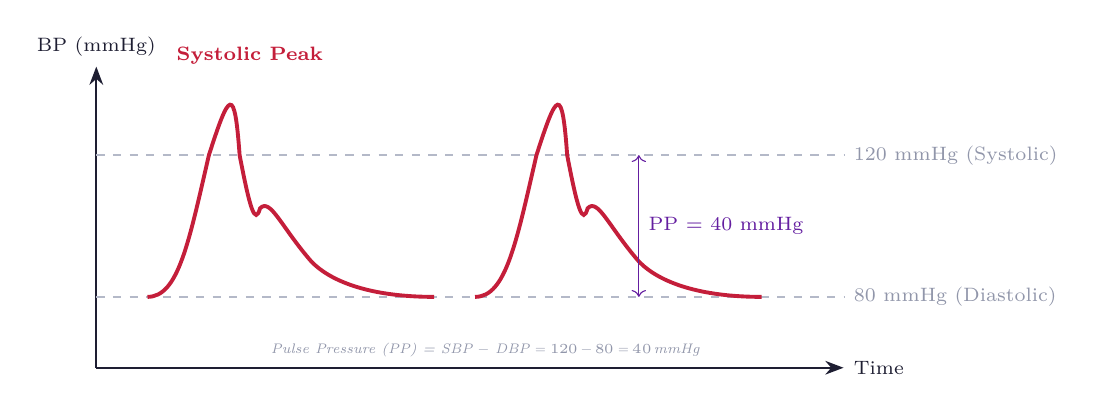
\begin{tikzpicture}[x=1.3cm, y=0.045cm, thick]
  \draw[arrow] (-0.3, 60) -- (-0.3, 145) node[above, font=\scriptsize] {BP (mmHg)};
  \draw[arrow] (-0.3, 60) -- (7.0, 60) node[right, font=\scriptsize] {Time};

  % Reference lines
  \draw[dashed, color=mgframe] (-0.3, 120) -- (7.0, 120) node[right, font=\scriptsize, color=watermark] {120 mmHg (Systolic)};
  \draw[dashed, color=mgframe] (-0.3, 80) -- (7.0, 80) node[right, font=\scriptsize, color=watermark] {80 mmHg (Diastolic)};

  % One cardiac cycle waveform, repeated twice
  \foreach \xoff in {0, 3.2} {
    \draw[color=myred, line width=1.4pt]
      (\xoff+0.2, 80)
      .. controls (\xoff+0.5, 80) and (\xoff+0.6, 95) .. (\xoff+0.8, 120)
      .. controls (\xoff+1.0, 138) and (\xoff+1.05, 140) .. (\xoff+1.1, 120)
      .. controls (\xoff+1.2, 105) and (\xoff+1.25, 100) .. (\xoff+1.3, 105)
      .. controls (\xoff+1.4, 108) and (\xoff+1.5, 100) .. (\xoff+1.8, 90)
      .. controls (\xoff+2.0, 84) and (\xoff+2.4, 80) .. (\xoff+3.0, 80);
  }

  % Labels
  \node[font=\scriptsize\bfseries, color=myred] at (1.2, 148) {Systolic Peak};
  \draw[<->, color=mypurple, thin] (5.0, 80) -- (5.0, 120) node[midway, right, font=\scriptsize, color=mypurple] {PP = 40 mmHg};

  % Annotation
  \node[font=\tiny\itshape, color=watermark] at (3.5, 65) {Pulse Pressure (PP) = SBP $-$ DBP $= 120-80 = 40\,\text{mmHg}$};
\end{tikzpicture}
\end{tcolorbox}

\textbf{Oscillometric Method (Automated NIBP monitors):} The cuff is inflated and deflated automatically. A pressure sensor in the monitor detects the oscillations of the arterial wall transmitted through the cuff. Maximum oscillation occurs at \textbf{MAP} (Mean Arterial Pressure). Systolic and diastolic pressures are computed algorithmically.

\begin{tcolorbox}[formulabox, title={\textbf{Blood Pressure Formulas}}]
\renewcommand{\arraystretch}{1.3}
\begin{tabularx}{\linewidth}{B{3.8cm} X}
Pulse Pressure & $PP = SBP - DBP = 120 - 80 = 40\,\text{mmHg}$ \\[4pt]
Mean Arterial Pressure & $MAP = DBP + \dfrac{PP}{3} = 80 + \dfrac{40}{3} \approx 93\,\text{mmHg}$ \\[8pt]
Alternatively & $MAP = \dfrac{SBP + 2 \times DBP}{3}$
\end{tabularx}
\end{tcolorbox}

% ===============================================================================
\section{Blood Flow Measurement}
% ===============================================================================

\subsection{Electromagnetic Flowmeter (Review)}

Based on Faraday's law: $V_{emf} = Bvd$ (covered in Module 2). Used intraoperatively to measure coronary or renal artery blood flow.

\subsection{Plethysmography}

\begin{tcolorbox}[defbox, title={\textbf{Plethysmography}}]
\textbf{Plethysmography} is the measurement of changes in \textbf{volume} of a body part or organ, used to assess blood flow and venous function. It detects volumetric pulsations caused by arterial inflow exceeding venous outflow during systole.
\end{tcolorbox}

\textbf{Types:} (a) \textbf{Strain-gauge plethysmography:} A mercury-in-silastic gauge around the limb stretches with each pulse, changing resistance $\propto$ volume change. (b) \textbf{Photo-plethysmography (PPG):} Light from an LED is transmitted through or reflected from the tissue; the varying absorption of the pulsatile blood volume modulates the photodetector output. Basis of pulse oximetry.

% ===============================================================================
\section{Impedance Plethysmography}
% ===============================================================================

\begin{tcolorbox}[defbox, title={\textbf{Impedance Plethysmography}}]
\textbf{Impedance plethysmography} measures changes in the \textbf{electrical impedance} of a body segment (typically the thorax or a limb) to infer changes in blood volume or respiratory activity. Blood has a lower resistivity than surrounding tissue, so arterial blood inflow during systole decreases the measured impedance.
\end{tcolorbox}

\subsection{Principle}

A high-frequency ($20$--$100\,\text{kHz}$), low-amplitude ($1$--$4\,\text{mA}$ rms) alternating current is injected through outer electrodes. The voltage is sensed by inner (pick-up) electrodes, and the impedance $Z = V/I$ is computed. Changes in blood volume produce small, rhythmic changes in impedance $\Delta Z$.

\subsection{Nyboer's Formula (Limb Blood Flow)}

\begin{tcolorbox}[formulabox, title={\textbf{Impedance Plethysmography Formulas}}]
\[
\Delta V = \frac{\rho_b \cdot L^2}{Z_0^2} \cdot \Delta Z
\]
where: $\Delta V$ = change in blood volume (mL), $\rho_b$ = resistivity of blood ($\approx 150\,\Omega\cdot\text{cm}$), $L$ = segment length (cm), $Z_0$ = baseline impedance ($\Omega$), $\Delta Z$ = impedance change ($\Omega$). \\[6pt]
\textbf{Impedance Cardiography (ICG)} measures stroke volume and cardiac output non-invasively from thoracic impedance changes.
\end{tcolorbox}

\begin{tcolorbox}[tikzbox, title={Impedance Plethysmography --- 4-Electrode Configuration}]
\centering
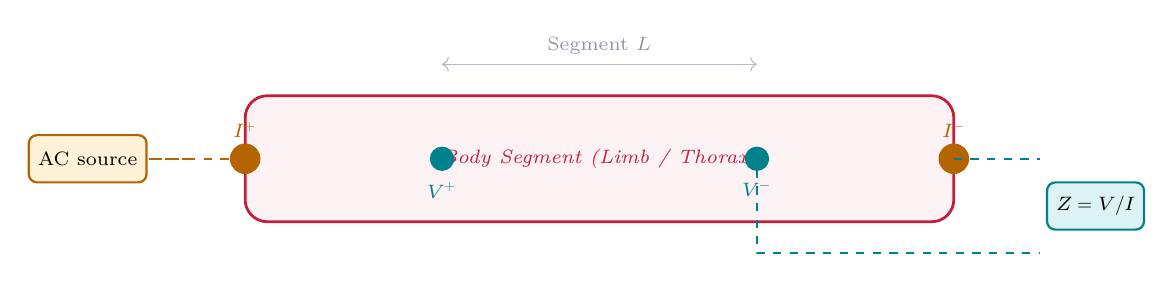
\begin{tikzpicture}[thick, font=\small]
  % Limb segment (rectangle)
  \filldraw[fill=hdrred!60, draw=myred, rounded corners=8pt, line width=1pt]
    (-4.5, -0.8) rectangle (4.5, 0.8);
  \node[font=\scriptsize\itshape, color=myred] at (0, 0) {Body Segment (Limb / Thorax)};

  % Outer current injection electrodes (I+ and I-)
  \filldraw[fill=myamber, draw=myamber] (-4.5, 0) circle (0.18) node[above=4pt, font=\scriptsize\bfseries, color=myamber] {$I^+$};
  \filldraw[fill=myamber, draw=myamber] (4.5, 0) circle (0.18) node[above=4pt, font=\scriptsize\bfseries, color=myamber] {$I^-$};

  % Inner voltage sense electrodes (V+ and V-)
  \filldraw[fill=myteal, draw=myteal] (-2.0, 0) circle (0.14) node[below=5pt, font=\scriptsize\bfseries, color=myteal] {$V^+$};
  \filldraw[fill=myteal, draw=myteal] (2.0, 0) circle (0.14) node[below=5pt, font=\scriptsize\bfseries, color=myteal] {$V^-$};

  % Current source (left)
  \draw[color=myamber, dashed] (-4.5, 0) -- (-5.8, 0);
  \node[draw=myamber, fill=hdramber, rounded corners=3pt, font=\scriptsize, minimum width=1.0cm, minimum height=0.6cm]
    at (-6.5, 0) {AC source};
  \draw[color=myamber, dashed] (-5.2, 0) -- (-5.8, 0);

  % Voltage sense amplifier (right)
  \draw[color=myteal, dashed] (4.5, 0) -- (5.6, 0);
  \draw[color=myteal, dashed] (2.0, -0.14) -- (2.0, -1.2) -- (5.6, -1.2);
  \node[draw=myteal, fill=hdrteal, rounded corners=3pt, font=\scriptsize, minimum width=1.2cm, minimum height=0.6cm]
    at (6.3, -0.6) {$Z = V/I$};

  % Spacing label
  \draw[<->, color=mgframe, thin] (-2.0, 1.2) -- (2.0, 1.2) node[midway, above, font=\scriptsize, color=watermark] {Segment $L$};
\end{tikzpicture}
\end{tcolorbox}

\textbf{Clinical Applications of Impedance Plethysmography:}
\begin{itemize}[leftmargin=*, itemsep=2pt]
  \item \textbf{Cardiac output} measurement (non-invasive impedance cardiography).
  \item \textbf{Respiratory rate and tidal volume} monitoring (thoracic impedance changes with breathing).
  \item \textbf{Deep Vein Thrombosis (DVT)} detection by venous occlusion impedance plethysmography.
  \item \textbf{Body composition analysis} (bioelectrical impedance analysis, BIA).
\end{itemize}

% ===============================================================================
\section{Ultrasonic Imaging}
% ===============================================================================

\begin{tcolorbox}[defbox, title={\textbf{Ultrasonic Imaging}}]
\textbf{Ultrasonic imaging} uses high-frequency sound waves ($1$--$20\,\text{MHz}$) generated by piezoelectric transducers to visualize internal body structures. Sound waves are reflected at tissue interfaces (impedance mismatch), and the time of return (echo) and amplitude are used to construct images.
\end{tcolorbox}

\subsection{Acoustic Impedance and Reflection}

\begin{tcolorbox}[formulabox, title={\textbf{Ultrasound Key Formulas}}]
\renewcommand{\arraystretch}{1.3}
\begin{tabularx}{\linewidth}{B{3.8cm} X}
Speed of sound in tissue & $c \approx 1540\,\text{m/s}$ (average soft tissue). \\[4pt]
Acoustic impedance & $Z = \rho \cdot c$ \quad ($\rho$ = density, kg/m$^3$) \\[4pt]
Reflection coefficient & $R = \left(\dfrac{Z_2 - Z_1}{Z_2 + Z_1}\right)^2$ \\[8pt]
Depth of reflector & $d = \dfrac{c \cdot t}{2}$ \quad ($t$ = round-trip travel time) \\[4pt]
Axial resolution & $\Delta z = \dfrac{c}{2B}$ \quad ($B$ = pulse bandwidth) \\[4pt]
Doppler shift & $\Delta f = \dfrac{2 f_0 v \cos\theta}{c}$
\end{tabularx}
\end{tcolorbox}

\subsection{Modes of Ultrasonic Imaging}

\par\noindent
\begin{tabularx}{\linewidth}{|B{2.0cm}|Y|Y|}
\hline
\textbf{Mode} & \textbf{\color{myteal}Description} & \textbf{\color{mygreen}Application} \\
\hline
A-mode (Amplitude) & Echoes displayed as amplitude spikes vs.\ time. 1D range measurement. & Ophthalmology (eye axial length); echoencephalography. \\
\hline
B-mode (Brightness) & Echo amplitude coded as brightness; 2D scan built by sweeping the beam. & Standard abdominal, obstetric ultrasound; liver, kidney, uterus. \\
\hline
M-mode (Motion) & Single beam; echoes displayed as position vs.\ time graph. Captures motion. & Echocardiography: cardiac valve motion, chamber dimension. \\
\hline
Doppler (Colour Flow) & Blood velocity colour-coded (red = towards, blue = away) overlaid on B-mode. & Vascular studies, cardiac valve regurgitation, stenosis. \\
\hline
3D / 4D & Multiple 2D planes reconstructed into 3D volume; 4D adds real-time motion. & Fetal morphology, cardiac volume assessment. \\
\hline
\end{tabularx}

\begin{tcolorbox}[tikzbox, title={Ultrasound Imaging System Block Diagram}]
\centering
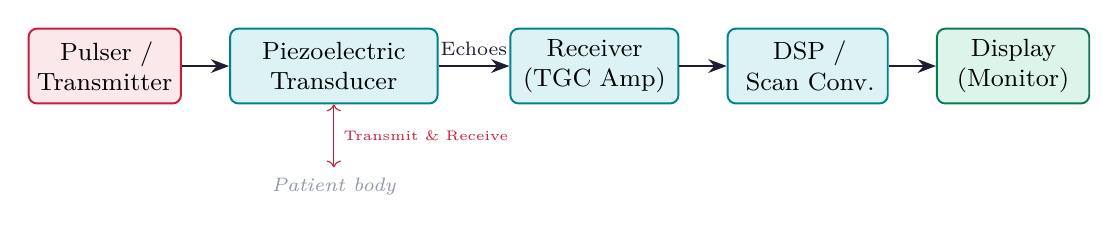
\begin{tikzpicture}[thick, font=\small,
  sblock/.style={rectangle, draw=myteal, fill=hdrteal,
    align=center, minimum height=0.95cm, font=\small,
    rounded corners=3pt, line width=0.7pt},
  spulser/.style={rectangle, draw=myred, fill=hdrred,
    align=center, minimum height=0.95cm, font=\small,
    rounded corners=3pt, line width=0.7pt},
  sdisp/.style={rectangle, draw=mygreen, fill=hdrgreen,
    align=center, minimum height=0.95cm, font=\small,
    rounded corners=3pt, line width=0.7pt}]

  \node[spulser, text width=1.7cm] (pulser) {Pulser /\\Transmitter};
  \node[sblock, right=0.6cm of pulser, text width=2.4cm] (xdcr) {Piezoelectric\\Transducer};
  \node[sblock, right=0.9cm of xdcr, text width=1.9cm] (recv) {Receiver\\(TGC Amp)};
  \node[sblock, right=0.6cm of recv, text width=1.8cm] (dsp) {DSP /\\Scan Conv.};
  \node[sdisp, right=0.6cm of dsp, text width=1.7cm] (disp) {Display\\(Monitor)};

  % Arrows
  \draw[arrow] (pulser) -- (xdcr);
  \draw[arrow] (xdcr) -- node[above, font=\scriptsize] {Echoes} (recv);
  \draw[arrow] (recv) -- (dsp);
  \draw[arrow] (dsp) -- (disp);

  % Body annotation
  \node[font=\scriptsize\itshape, color=watermark, below=0.8cm of xdcr] (body) {Patient body};
  \draw[<->, color=myred, thin] (xdcr.south) -- (body.north) node[midway, right, font=\tiny, color=myred] {Transmit \& Receive};
\end{tikzpicture}
\end{tcolorbox}

\textbf{Time-Gain Compensation (TGC):} Echoes from deeper structures are weaker due to attenuation. TGC amplifies echoes by an increasing gain as a function of time (depth) to equalize the displayed brightness across depth. Typical attenuation: $\approx 0.5\,\text{dB/cm/MHz}$.

% ===============================================================================
\section{X-ray Imaging}
% ===============================================================================

\begin{tcolorbox}[defbox, title={\textbf{X-ray Imaging}}]
\textbf{X-rays} are electromagnetic radiation ($0.01$--$10\,\text{nm}$ wavelength; $10^{16}$--$10^{19}\,\text{Hz}$) generated by bombarding a tungsten anode with high-velocity electrons. They penetrate tissue differentially based on tissue density and atomic number, creating a projected shadow image.
\end{tcolorbox}

\subsection{Attenuation Law}

\begin{tcolorbox}[formulabox, title={\textbf{Beer-Lambert Law for X-rays}}]
\[
I = I_0 \cdot e^{-\mu x}
\]
where $I_0$ = incident X-ray intensity, $I$ = transmitted intensity, $\mu$ = linear attenuation coefficient (cm$^{-1}$, depends on material and photon energy), $x$ = thickness of material (cm).
\end{tcolorbox}

\textbf{Tissue Contrast:} Bone ($\mu$ high, appears white) $>$ Soft tissue $>$ Fat $>$ Air ($\mu$ low, appears black).

\subsection{Computed Tomography (CT)}

\begin{tcolorbox}[defbox, title={\textbf{Computed Tomography (CT)}}]
\textbf{CT} (Computerised Tomography, or CAT scan) uses a rotating X-ray source and a detector array to acquire many projections at different angles. A reconstruction algorithm (\textbf{filtered back-projection} or iterative methods) produces cross-sectional (axial) images of the body. CT values are expressed in \textbf{Hounsfield Units (HU)}: water $= 0\,\text{HU}$, air $= -1000\,\text{HU}$, bone $= +400$ to $+1000\,\text{HU}$.
\end{tcolorbox}

\textbf{Advantages of CT over plain X-ray:} Cross-sectional images eliminate overlapping structures; better soft tissue contrast with contrast agents; enables 3D reconstruction.

\textbf{Radiation dose:} CT delivers a significantly higher dose than plain X-ray (chest CT $\approx 7\,\text{mSv}$ vs.\ chest X-ray $\approx 0.1\,\text{mSv}$).

% ===============================================================================
\section{Nuclear Imaging}
% ===============================================================================

\begin{tcolorbox}[defbox, title={\textbf{Nuclear (Radionuclide) Imaging}}]
\textbf{Nuclear imaging} introduces a radioactive tracer (\textbf{radiopharmaceutical}) into the patient. The tracer accumulates in target tissues (e.g., tumour, heart). Gamma rays emitted by the tracer are detected externally to create functional images showing organ physiology and metabolism rather than anatomy alone.
\end{tcolorbox}

\subsection{Scintigraphy and Gamma Camera}

A radiotracer (e.g., Technetium-99m, $^{99m}$Tc, emitting $140\,\text{keV}$ gamma rays) is injected. The \textbf{gamma camera (Anger camera)} uses a large NaI(Tl) scintillator crystal coupled to an array of photomultiplier tubes (PMTs) to detect and locate each gamma photon. A collimator ensures only perpendicularly incident photons reach the crystal. The image represents tracer distribution in the organ.

\subsection{SPECT (Single Photon Emission Computed Tomography)}

A gamma camera rotates around the patient, acquiring multiple projections. 3D images are reconstructed similarly to CT. Used for: myocardial perfusion imaging (heart), brain SPECT (epilepsy, dementia), bone scans.

\subsection{PET (Positron Emission Tomography)}

\begin{tcolorbox}[defbox, title={\textbf{PET Scanning}}]
\textbf{PET} uses positron-emitting radiotracers (e.g., $^{18}$F-FDG, a glucose analogue). The emitted positron annihilates with an electron, producing two $511\,\text{keV}$ gamma photons travelling in \textbf{opposite directions} ($180^{\circ}$). Coincidence detection of both photons defines the line of response without a collimator, giving higher sensitivity and resolution than SPECT.
\end{tcolorbox}

\par\noindent
\begin{tabularx}{\linewidth}{|B{2.2cm}|Y|Y|Y|}
\hline
\textbf{Technique} & \textbf{\color{myteal}Radiation} & \textbf{\color{myamber}Resolution} & \textbf{\color{mygreen}Key Application} \\
\hline
\textbf{X-ray} & X-ray photons & 0.1 mm & Bone fractures, chest pathology. \\
\hline
\textbf{CT} & X-ray photons & 0.5--1 mm & Trauma, lung, abdominal, 3D anatomy. \\
\hline
\textbf{Scintigraphy} & $\gamma$ rays (single) & 10--15 mm & Bone scans, thyroid function. \\
\hline
\textbf{SPECT} & $\gamma$ rays (single) & 7--10 mm & Cardiac perfusion, brain function. \\
\hline
\textbf{PET} & $\gamma$ rays (coincidence) & 3--5 mm & Oncology (tumour), brain metabolism. \\
\hline
\textbf{PET-CT} & Combined & 3--5 mm & Anatomy + Function fusion; gold standard in oncology. \\
\hline
\end{tabularx}

\newpage
% ===============================================================================
% MANDATORY QUICK REVISION PAGE
% ===============================================================================
\begin{center}
  {\large\bfseries\color{myred} Quick Revision --- Module 3}\\[3pt]
  {\small\color{mydark} Physiological Measurement and Medical Imaging $|$ PE-EC603B}
\end{center}
\noindent{\color{myred}\rule{\linewidth}{1.2pt}}
\vspace{4pt}

\begin{tcolorbox}[formulabox, title={\textbf{Key Formulas}}]
\renewcommand{\arraystretch}{1.3}
\begin{tabularx}{\linewidth}{B{4.0cm} X}
Mean Arterial Pressure & $MAP = DBP + PP/3 = (SBP + 2\,DBP)/3$ \\[4pt]
Pulse Pressure & $PP = SBP - DBP$ \\[4pt]
Thermodilution CO & $CO = \dfrac{V_{inj}(T_B - T_{inj})\cdot K}{\int \Delta T_B\,dt}$ \\[8pt]
Impedance plethysm. & $\Delta V = \dfrac{\rho_b L^2}{Z_0^2}\Delta Z$ \\[8pt]
Ultrasound depth & $d = ct/2$ \\[4pt]
Acoustic impedance & $Z = \rho c$ \\[4pt]
Reflection coeff. & $R = \left(\dfrac{Z_2-Z_1}{Z_2+Z_1}\right)^2$ \\[8pt]
X-ray attenuation & $I = I_0 e^{-\mu x}$ \\[4pt]
Doppler shift & $\Delta f = 2f_0 v\cos\theta / c$
\end{tabularx}
\end{tcolorbox}

\begin{tcolorbox}[defbox, title={\textbf{One-Line Definitions}}]
\begin{itemize}[leftmargin=*, itemsep=2.5pt, topsep=0pt]
  \item \textbf{Korotkoff Sounds:} Sounds heard through a stethoscope during sphygmomanometer BP measurement; first sound = systolic BP; disappearance = diastolic BP.
  \item \textbf{Pulse Pressure:} Difference between systolic and diastolic BP ($\approx 40\,\text{mmHg}$).
  \item \textbf{Impedance Plethysmography:} Measures blood volume changes via electrical impedance changes of a body segment.
  \item \textbf{TGC (Time-Gain Compensation):} Increasing amplifier gain with time to compensate for ultrasound attenuation at greater depths.
  \item \textbf{Acoustic Impedance:} Product of tissue density and sound velocity ($Z = \rho c$); mismatch between tissues causes ultrasound reflection.
  \item \textbf{Hounsfield Unit:} Standardized scale of X-ray attenuation in CT; water = 0 HU, air = $-1000$ HU.
  \item \textbf{Scintigraphy:} 2D nuclear imaging using a gamma camera after radiopharmaceutical injection.
  \item \textbf{PET:} Positron Emission Tomography; uses annihilation coincidence detection of two $511\,\text{keV}$ photons for 3D functional imaging.
  \item \textbf{A-mode ultrasound:} One-dimensional distance measurement from echo amplitude spikes on a time axis.
  \item \textbf{B-mode ultrasound:} 2D grey-scale image formed by brightness-coding echo amplitude as the beam is swept.
\end{itemize}
\end{tcolorbox}

\begin{tcolorbox}[exambox, title={\textbf{Frequently Asked / Viva Questions}}]
\begin{enumerate}[topsep=0pt, label=\textbf{Q\arabic*.}, itemsep=5pt]
  \item \Q{Describe the Korotkoff sound method for non-invasive blood pressure measurement.}
    A cuff is inflated above systolic pressure (artery occluded; no sound). As cuff deflates, the first tapping Korotkoff sound marks \textit{systolic BP}. Sounds change character until they disappear entirely at \textit{diastolic BP}, when the artery is fully open.
  \item \Q{What is the oscillometric method of blood pressure measurement?}
    An automated cuff inflates and deflates. A pressure sensor detects oscillations from the arterial wall transmitted through cuff air. Maximum oscillation amplitude occurs at MAP. Systolic and diastolic pressures are computed by algorithm from the oscillation envelope.
  \item \Q{Define Mean Arterial Pressure and give its formula.}
    MAP is the average arterial pressure over one cardiac cycle, weighted for the longer diastolic phase: $MAP = DBP + PP/3 \approx 93\,\text{mmHg}$. Alternatively $MAP = (SBP + 2\times DBP)/3$.
  \item \Q{What is impedance plethysmography? State the Nyboer formula.}
    It measures blood volume changes by injecting a safe high-frequency AC current and detecting impedance changes: $\Delta V = \rho_b L^2 \Delta Z / Z_0^2$. Arterial inflow during systole decreases impedance; respiratory motion also changes thoracic impedance.
  \item \Q{Explain acoustic impedance and its role in ultrasound imaging.}
    Acoustic impedance $Z = \rho c$. At the boundary between tissues with different $Z$, a fraction of the ultrasound energy is reflected: $R = [(Z_2-Z_1)/(Z_2+Z_1)]^2$. These reflections (echoes) form the image. At air--tissue interfaces, nearly all energy is reflected ($R \approx 1$), which is why coupling gel is essential.
  \item \Q{Compare A-mode, B-mode, and M-mode ultrasound.}
    A-mode: amplitude spikes vs.\ time for 1D depth measurement (e.g., eye). B-mode: 2D brightness map used in standard diagnostic ultrasound (abdomen, obstetrics). M-mode: single beam traces target motion over time (e.g., cardiac valve motion).
  \item \Q{State the Beer-Lambert law for X-rays and explain Hounsfield Units.}
    $I = I_0 e^{-\mu x}$. In CT, the Hounsfield Unit (HU) normalizes attenuation: water $= 0\,\text{HU}$, air $= -1000\,\text{HU}$, bone $= +400$ to $+1000\,\text{HU}$. It enables standardized comparison between scanners.
  \item \Q{What is the principle of PET scanning? How does it differ from SPECT?}
    PET uses positron-emitting tracers (e.g., $^{18}$F-FDG). Each positron annihilates with an electron to emit two $511\,\text{keV}$ photons at $180^{\circ}$. Coincidence detection defines the line of response without a collimator, giving higher sensitivity and resolution ($3$--$5\,\text{mm}$). SPECT uses a single-photon emitter and a mechanical collimator, giving lower resolution ($7$--$10\,\text{mm}$) but lower cost.
  \item \Q{Why is TGC (Time-Gain Compensation) needed in ultrasound?}
    Ultrasound is attenuated as it travels through tissue ($\approx 0.5\,\text{dB/cm/MHz}$). Deeper echoes return later and are weaker. TGC progressively increases amplifier gain with time (depth) to compensate, so that interfaces at all depths appear equally bright on the display.
  \item \Q{What is thermodilution and what does it measure?}
    Thermodilution measures cardiac output. Cold saline is injected into the right atrium; a thermistor in the pulmonary artery detects the temperature--time curve. By the Stewart-Hamilton equation, cardiac output is inversely proportional to the area under the temperature-change curve: $CO \propto 1/\int \Delta T_B\,dt$.
\end{enumerate}
\end{tcolorbox}

\begin{tcolorbox}[tikzbox, title={Imaging Modality Comparison}]
\renewcommand{\arraystretch}{1.4}
\par\noindent
\begin{tabularx}{\linewidth}{|B{2.0cm}|>{\small\centering\arraybackslash}X|>{\small\centering\arraybackslash}X|>{\small\centering\arraybackslash}X|>{\small\centering\arraybackslash}X|Y|}
\hline
\textbf{Modality} & \textbf{\color{myred}Ionizing?} & \textbf{\color{myteal}Resolution} & \textbf{\color{myamber}Image type} & \textbf{\color{mypurple}Real-time?} & \textbf{Best for} \\
\hline
X-ray & Yes & 0.1 mm & 2D shadow & No & Bone, chest \\
\hline
CT & Yes & 0.5 mm & 3D slices & No & Trauma, anatomy \\
\hline
Ultrasound & No & 0.5--2 mm & 2D/3D & Yes & Soft tissue, fetus \\
\hline
SPECT & Yes & 7--10 mm & 3D functional & No & Cardiac perfusion \\
\hline
PET & Yes & 3--5 mm & 3D metabolic & No & Oncology, brain \\
\hline
MRI & No & 0.5--1 mm & 3D anatomy & No & Brain, soft tissue \\
\hline
\end{tabularx}
\end{tcolorbox}


% -- Module 4 -----------------------------------------------------------------
\modulestart{4}{Cardiac Pacemakers}

\section{Cardiac Pacemakers}
% ===============================================================================

\begin{tcolorbox}[defbox, title={\textbf{Definition: Cardiac Pacemaker}}]
A \textbf{cardiac pacemaker} is an implantable electronic device that delivers controlled electrical stimuli to the heart muscle to maintain an adequate heart rate when the natural conduction system (SA node, AV node) fails or is too slow (bradycardia, heart block, sick sinus syndrome).
\end{tcolorbox}

\subsection{Pacemaker Block Diagram}

\begin{tcolorbox}[tikzbox, title={Cardiac Pacemaker Block Diagram}]
\centering
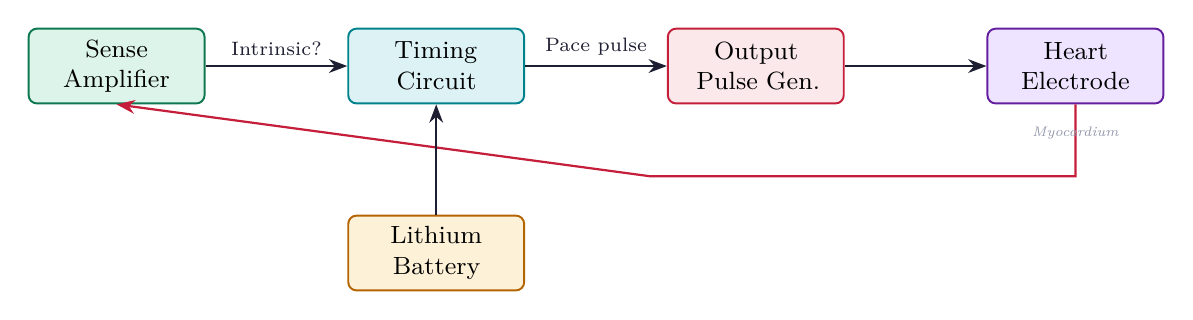
\begin{tikzpicture}[node distance=0.7cm and 1.6cm, thick, font=\small]
  % Sense
  \node[greenblock, text width=2.0cm] (sense) {Sense\\Amplifier};
  % Timing
  \node[block, text width=2.0cm, right=1.8cm of sense] (timing) {Timing\\Circuit};
  % Output
  \node[redblock, text width=2.0cm, right=1.8cm of timing] (output) {Output\\Pulse Gen.};
  % Battery
  \node[amberblock, text width=2.0cm, below=1.4cm of timing] (batt) {Lithium\\Battery};
  % Lead/electrode
  \node[purpblock, text width=2.0cm, right=1.8cm of output] (heart) {Heart\\Electrode};

  % Arrows
  \draw[arrow] (sense) -- node[above, font=\scriptsize] {Intrinsic?} (timing);
  \draw[arrow] (timing) -- node[above, font=\scriptsize] {Pace pulse} (output);
  \draw[arrow] (output) -- (heart);
  \draw[redarrow] (heart) -- ++(0,-1.4) -- ++(-5.4,0) -- (sense.south);
  \draw[arrow] (batt) -- (timing);
  \node[font=\tiny\itshape, color=watermark, below=0.15cm of heart] {Myocardium};
\end{tikzpicture}
\end{tcolorbox}

\subsection{Types of Pacemakers}

\par\noindent
\begin{tabularx}{\linewidth}{|B{2.8cm}|Y|Y|}
\hline
\textbf{Type} & \textbf{\color{myteal}Description} & \textbf{\color{mygreen}Use} \\
\hline
\textbf{Single-chamber (AAI / VVI)} & Senses and paces one chamber only (atrium or ventricle). & Sick sinus syndrome (AAI); complete heart block (VVI). \\
\hline
\textbf{Dual-chamber (DDD)} & Senses and paces both atrium and ventricle; maintains AV synchrony. & AV block with intact SA node. \\
\hline
\textbf{Rate-responsive (DDDR)} & Uses sensor (accelerometer, minute ventilation) to increase rate during exercise. & Chronotropic incompetence, active patients. \\
\hline
\textbf{CRT (Biventricular)} & Paces both ventricles simultaneously to resynchronize contraction. & Heart failure with left bundle branch block. \\
\hline
\textbf{Leadless pacemaker} & Capsule implanted directly in right ventricle; no transvenous lead. & Single-chamber pacing without lead complications. \\
\hline
\end{tabularx}

\subsection{Pacemaker Timing Parameters}

\begin{tcolorbox}[formulabox, title={\textbf{Pacemaker Timing Intervals}}]
\renewcommand{\arraystretch}{1.3}
\begin{tabularx}{\linewidth}{B{3.8cm} X}
Pacing Rate & $\text{Rate (bpm)} = \dfrac{60\,000}{\text{Pacing Interval (ms)}}$ \\[8pt]
AV Delay & Time from atrial pace/sense to ventricular pace ($\approx 120$--$200\,\text{ms}$; mimics PR interval). \\[4pt]
Refractory Period & Time after a sensed/paced event during which the pacemaker ignores signals ($\approx 250$--$400\,\text{ms}$). \\[4pt]
Escape Interval & Time from a sensed beat to the next paced beat if no intrinsic beat occurs. \\[4pt]
Pulse Width & Duration of pacing pulse ($\approx 0.4$--$1.0\,\text{ms}$). \\[4pt]
Pulse Amplitude & Voltage of pacing pulse ($\approx 2.5$--$5\,\text{V}$; must exceed stimulation threshold).
\end{tabularx}
\end{tcolorbox}

\textbf{Energy Source:} Lithium--iodide (LiI) battery; longevity $5$--$15$ years. Elective Replacement Indicator (ERI) detects end-of-battery voltage ($2.4\,\text{V}$ from $2.8\,\text{V}$ nominal).

% ===============================================================================
\section{Defibrillators}
% ===============================================================================

\begin{tcolorbox}[defbox, title={\textbf{Definition: Defibrillator}}]
A \textbf{defibrillator} is a device that delivers a controlled, high-energy electrical shock to the heart to terminate life-threatening arrhythmias such as \textbf{ventricular fibrillation (VF)} and \textbf{ventricular tachycardia (VT)}, depolarizing all cardiac cells simultaneously so that the SA node can resume normal pacemaker control.
\end{tcolorbox}

\subsection{Principle and Types}

\textbf{Ventricular fibrillation} is chaotic, uncoordinated cardiac electrical activity --- the heart quivers rather than pumping. Without defibrillation within $\approx 4$--$6\,\text{minutes}$, brain death ensues.

\par\noindent
\begin{tabularx}{\linewidth}{|B{3.0cm}|Y|Y|}
\hline
\textbf{Type} & \textbf{\color{myteal}Description} & \textbf{\color{mygreen}Energy} \\
\hline
\textbf{External} & Paddle or adhesive pad electrodes on chest wall. & 150--360 J (monophasic); 120--200 J (biphasic). \\
\hline
\textbf{Internal} & Used during cardiac surgery; paddles placed directly on heart. & 20--50 J. \\
\hline
\textbf{ICD (Implantable Cardioverter Defibrillator)} & Permanently implanted; monitors rhythm continuously; delivers therapy automatically. & 25--40 J; also provides anti-tachycardia pacing. \\
\hline
\textbf{AED (Automated External Defibrillator)} & Portable; analyses rhythm and advises/delivers shock automatically. Designed for lay-rescuer use. & 120--200 J (biphasic). \\
\hline
\end{tabularx}

\subsection{Defibrillator Circuit and Waveforms}

\begin{tcolorbox}[tikzbox, title={Defibrillator Discharge Circuit and Waveforms}]
\centering
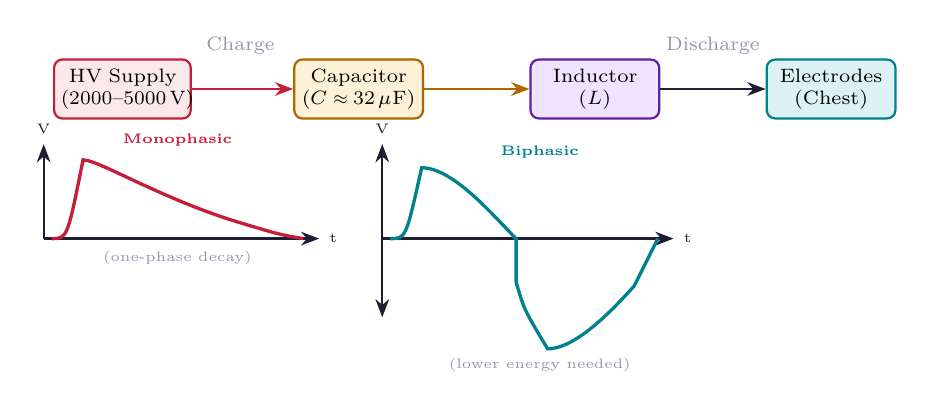
\begin{tikzpicture}[thick, font=\small]
  % --- Circuit ---
  % Capacitor charging from high-voltage supply
  \node[draw=myred, fill=hdrred, rounded corners=3pt,
        minimum width=1.6cm, minimum height=0.7cm, font=\scriptsize,
        align=center, text width=1.5cm] (hv) at (-4.5, 2.0) {HV Supply\\{\scriptsize(2000--5000\,V)}};
  \node[draw=myamber, fill=hdramber, rounded corners=3pt,
        minimum width=1.4cm, minimum height=0.7cm, font=\scriptsize,
        align=center, text width=1.4cm] (cap) at (-1.5, 2.0) {Capacitor\\{\scriptsize($C \approx 32\,\mu\text{F}$)}};
  \node[draw=mypurple, fill=hdrpurple, rounded corners=3pt,
        minimum width=1.4cm, minimum height=0.7cm, font=\scriptsize,
        align=center, text width=1.4cm] (ind) at (1.5, 2.0) {Inductor\\($L$)};
  \node[draw=myteal, fill=hdrteal, rounded corners=3pt,
        minimum width=1.4cm, minimum height=0.7cm, font=\scriptsize,
        align=center, text width=1.4cm] (pad) at (4.5, 2.0) {Electrodes\\{\scriptsize(Chest)}};

  \draw[arrow, color=myred] (hv) -- (cap);
  \draw[arrow, color=myamber] (cap) -- (ind);
  \draw[arrow] (ind) -- (pad);

  \node[font=\scriptsize, color=watermark] at (-3.0, 2.55) {Charge};
  \node[font=\scriptsize, color=watermark] at (3.0, 2.55) {Discharge};

  % --- Waveform comparison ---
  \begin{scope}[yshift=-0.4cm]
    % Monophasic axis
    \draw[arrow] (-5.5, 0.5) -- (-2.0, 0.5) node[right, font=\tiny] {t};
    \draw[arrow] (-5.5, 0.5) -- (-5.5, 1.7) node[above, font=\tiny] {V};
    \draw[color=myred, line width=1.2pt] (-5.4, 0.5)
      .. controls (-5.2,0.5) .. (-5.0, 1.5)
      .. controls (-4.8,1.5) and (-4.0, 1.0) .. (-3.0, 0.7)
      .. controls (-2.5, 0.55) .. (-2.2, 0.5);
    \node[font=\tiny\bfseries, color=myred] at (-3.8, 1.75) {Monophasic};
    \node[font=\tiny, color=watermark] at (-3.8, 0.25) {(one-phase decay)};

    % Biphasic axis
    \draw[arrow] (-1.2, 0.5) -- (2.5, 0.5) node[right, font=\tiny] {t};
    \draw[arrow] (-1.2, 0.5) -- (-1.2, 1.7) node[above, font=\tiny] {V};
    \draw[arrow] (-1.2, 0.5) -- (-1.2, -0.5);
    \draw[color=myteal, line width=1.2pt] (-1.1, 0.5)
      .. controls (-0.9, 0.5) .. (-0.7, 1.4)
      .. controls (-0.3, 1.4) and (0.2, 0.8) .. (0.5, 0.5)
      -- (0.5, -0.05)
      .. controls (0.6, -0.4) .. (0.9, -0.9)
      .. controls (1.2, -0.9) and (1.6, -0.55) .. (2.0, -0.1)
      -- (2.3, 0.5);
    \node[font=\tiny\bfseries, color=myteal] at (0.8, 1.6) {Biphasic};
    \node[font=\tiny, color=watermark] at (0.8, -1.1) {(lower energy needed)};
  \end{scope}
\end{tikzpicture}
\end{tcolorbox}

\textbf{Energy stored in capacitor:} $E = \dfrac{1}{2}CV^2$. For $C = 32\,\mu\text{F}$ and $V = 3000\,\text{V}$: $E = \dfrac{1}{2}\times 32\times10^{-6}\times(3000)^2 = 144\,\text{J}$.

\textbf{Biphasic vs.\ Monophasic:} Biphasic waveforms reverse polarity partway through the shock. They are more effective at lower energies ($\approx 150$--$200\,\text{J}$ vs.\ $360\,\text{J}$) and cause less myocardial injury. All modern defibrillators use biphasic waveforms.

% ===============================================================================
\section{Heart-Lung Machine (Cardiopulmonary Bypass)}
% ===============================================================================

\begin{tcolorbox}[defbox, title={\textbf{Heart-Lung Machine}}]
The \textbf{heart-lung machine} (cardiopulmonary bypass pump, CPB) temporarily takes over the function of the heart and lungs during open-heart surgery. It oxygenates blood, removes carbon dioxide, and pumps it back to the body, allowing surgeons to operate on a still, bloodless heart.
\end{tcolorbox}

\subsection{Components and Operation}

\begin{tcolorbox}[tikzbox, title={Cardiopulmonary Bypass Circuit}]
\centering
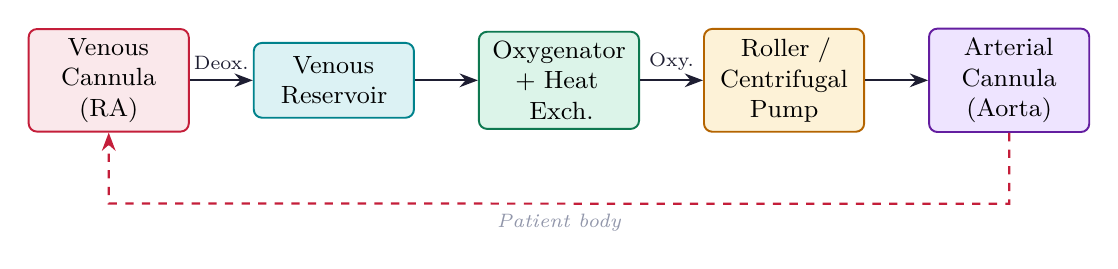
\begin{tikzpicture}[
  node distance=0.8cm and 0.8cm, thick, font=\small,
  sredblock/.style={rectangle, draw=myred, fill=hdrred, text width=1.8cm, align=center, minimum height=0.95cm, rounded corners=3pt, line width=0.7pt},
  sblock/.style={rectangle, draw=myteal, fill=hdrteal, text width=1.8cm, align=center, minimum height=0.95cm, rounded corners=3pt, line width=0.7pt},
  sgreenblock/.style={rectangle, draw=mygreen, fill=hdrgreen, text width=1.8cm, align=center, minimum height=0.95cm, rounded corners=3pt, line width=0.7pt},
  samberblock/.style={rectangle, draw=myamber, fill=hdramber, text width=1.8cm, align=center, minimum height=0.95cm, rounded corners=3pt, line width=0.7pt},
  spurpblock/.style={rectangle, draw=mypurple, fill=hdrpurple, text width=1.8cm, align=center, minimum height=0.95cm, rounded corners=3pt, line width=0.7pt}
]
  % Nodes
  \node[sredblock] (ra) {Venous\\Cannula\\(RA)};
  \node[sblock, right=0.8cm of ra] (resvr) {Venous\\Reservoir};
  \node[sgreenblock, right=0.8cm of resvr] (oxyg) {Oxygenator\\+ Heat Exch.};
  \node[samberblock, right=0.8cm of oxyg] (pump) {Roller /\\Centrifugal\\Pump};
  \node[spurpblock, right=0.8cm of pump] (ao) {Arterial\\Cannula\\(Aorta)};

  % Arrows
  \draw[arrow] (ra) -- node[above, font=\scriptsize] {Deox.} (resvr);
  \draw[arrow] (resvr) -- (oxyg);
  \draw[arrow] (oxyg) -- node[above, font=\scriptsize] {Oxy.} (pump);
  \draw[arrow] (pump) -- (ao);

  % Body loop at bottom
  \draw[redarrow, dashed] (ao.south) -- ++(0,-0.9) -- ($(ra.south)+(0,-0.9)$) node[midway, below, font=\scriptsize\itshape, color=watermark] {Patient body} -- (ra.south);
\end{tikzpicture}
\end{tcolorbox}

\textbf{Key components:}
\begin{itemize}[leftmargin=*, itemsep=3pt]
  \item \textbf{Oxygenator (Membrane type):} Blood flows past a semipermeable membrane; O$_2$ diffuses in and CO$_2$ diffuses out. Replaces the lungs.
  \item \textbf{Roller Pump / Centrifugal Pump:} Provides non-pulsatile (roller) or pulsatile (centrifugal) blood flow. Replaces the heart.
  \item \textbf{Heat Exchanger:} Lowers body temperature (hypothermia, $28$--$32\,^{\circ}$C) during surgery to reduce metabolic demand; rewarms blood before weaning from bypass.
  \item \textbf{Arterial Filter:} Removes air bubbles and particulate emboli from the arterial return line.
  \item \textbf{Cardioplegia system:} Cold potassium-rich solution delivered to coronary arteries to arrest the heart in diastole (electromechanical quiescence).
\end{itemize}

% ===============================================================================
\section{Artificial Kidney (Dialysis)}
% ===============================================================================

\begin{tcolorbox}[defbox, title={\textbf{Haemodialysis (Artificial Kidney)}}]
\textbf{Haemodialysis} is a renal replacement therapy for patients with End-Stage Renal Disease (ESRD). Blood is withdrawn, passed through a \textbf{dialyser} (artificial kidney) containing a semipermeable membrane, and returned to the body. The dialyser removes metabolic waste products (urea, creatinine, excess electrolytes) and excess water by the processes of \textbf{diffusion} and \textbf{ultrafiltration}.
\end{tcolorbox}

\subsection{Principles of Dialysis}

\begin{tcolorbox}[formulabox, title={\textbf{Mass Transport Mechanisms in Haemodialysis}}]
\renewcommand{\arraystretch}{1.3}
\begin{tabularx}{\linewidth}{B{3.2cm} X}
Diffusion & Movement of solutes across membrane from high to low concentration. Main mechanism for small solutes (urea, creatinine, potassium). \\[4pt]
Ultrafiltration & Hydraulic pressure drives water (and dissolved solutes) across the membrane. Controlled to remove excess fluid ($1$--$3\,\text{L/session}$). \\[4pt]
Clearance ($K$) & $K = \dfrac{Q_{Bi} \cdot C_{Bi} - Q_{Bo} \cdot C_{Bo}}{C_{Bi}}$ \quad (mL/min) \\[8pt]
KT/V & Urea dialysis adequacy measure: $Kt/V = -\ln(R - 0.008t) + (4-3.5R)\times\dfrac{UF}{W}$ \quad target $\geq 1.2$.
\end{tabularx}
\end{tcolorbox}

\subsection{Haemodialysis Circuit}

Blood is withdrawn from a vascular access (arteriovenous fistula, graft, or central venous catheter), anticoagulated with heparin, pumped through the dialyser at $200$--$500\,\text{mL/min}$ and returned. The dialysate (purified water + electrolytes) flows counter-current to blood at $500$--$800\,\text{mL/min}$.

\textbf{Safety alarms in a dialysis machine:}
\begin{itemize}[leftmargin=*, itemsep=2pt]
  \item Air bubble detector (ultrasonic).
  \item Venous pressure monitor (clot detection).
  \item Blood leak detector (photometric --- detects red blood cells in dialysate).
  \item Conductivity monitor (ensures correct dialysate concentration).
  \item Temperature alarm ($\pm 1\,^{\circ}$C from $37\,^{\circ}$C).
\end{itemize}

\textbf{Peritoneal Dialysis (PD):} Dialysate is instilled into the peritoneal (abdominal) cavity; the peritoneal membrane acts as the dialyser. No blood circuit required; performed at home. Less efficient than haemodialysis but better for residual renal function preservation.

% ===============================================================================
\section{Aids for the Handicapped}
% ===============================================================================

\subsection{Cochlear Implant}

\begin{tcolorbox}[defbox, title={\textbf{Cochlear Implant}}]
A \textbf{cochlear implant} is an electronic device that bypasses damaged hair cells in the cochlea and directly stimulates the auditory nerve fibres with electrical impulses, enabling profoundly deaf or severely hard-of-hearing individuals to perceive sound.
\end{tcolorbox}

\textbf{Components:}
\begin{enumerate}[leftmargin=*, itemsep=3pt]
  \item \textbf{Microphone} --- picks up sound from environment.
  \item \textbf{Speech Processor} (external, worn behind the ear) --- digitizes and filters sound into frequency bands; encodes into stimulation commands.
  \item \textbf{Transmitter Coil} (external) --- sends encoded signals transcutaneously via radiofrequency link to the internal receiver.
  \item \textbf{Internal Receiver/Stimulator} (implanted under skin) --- decodes RF signal, generates electrical pulses.
  \item \textbf{Electrode Array} (implanted in cochlea) --- 12--22 electrodes arranged tonotopically; each electrode stimulates a different frequency region of the auditory nerve.
\end{enumerate}

\subsection{Prosthetic Limbs}

\par\noindent
\begin{tabularx}{\linewidth}{|B{2.8cm}|Y|Y|}
\hline
\textbf{Type} & \textbf{\color{myteal}Control Mechanism} & \textbf{\color{mygreen}Application} \\
\hline
\textbf{Passive prosthesis} & Cosmetic only; no powered movement. & Upper/lower limb amputation cosmetic restoration. \\
\hline
\textbf{Body-powered} & Harness and cable system; shoulder/elbow movement activates hook or hand. & Upper limb; robust, low cost, proprioceptive feedback. \\
\hline
\textbf{Myoelectric (EMG-controlled)} & Surface EMG from residual muscles controls motor-driven hand/elbow. & Upper limb; intuitive control; electrically powered. \\
\hline
\textbf{Microprocessor knee} & Sensors and microcontroller adjust damping in real time for variable gait. & Trans-femoral (above-knee) amputation. \\
\hline
\end{tabularx}

\subsection{Other Assistive Devices}

\begin{itemize}[leftmargin=*, itemsep=3pt]
  \item \textbf{Visual prosthesis (Bionic eye):} Electrode array on retina or visual cortex stimulated by camera-processed signals to restore partial vision.
  \item \textbf{Deep Brain Stimulator (DBS):} Electrodes implanted in subthalamic nucleus; high-frequency ($130$--$180\,\text{Hz}$) electrical stimulation treats Parkinson's disease tremor.
  \item \textbf{Functional Electrical Stimulation (FES):} External electrodes stimulate paralysed muscles in paraplegic patients for assisted hand grasp or standing.
  \item \textbf{Hearing Aid:} Amplifies sound; does not bypass cochlea (unlike cochlear implant). Uses Class D amplifiers; ITE (in-the-ear) or BTE (behind-the-ear) form factors.
\end{itemize}

% ===============================================================================
\section{Electrical Safety in Medical Environments}
% ===============================================================================

\begin{tcolorbox}[defbox, title={\textbf{Importance of Electrical Safety}}]
Medical instruments are directly connected to or in close contact with patients. Even small leakage currents that are harmless in everyday life can be lethal in medical situations where electrodes bypass skin resistance or are in contact with the heart. Electrical safety standards (IEC 60601) define acceptable limits to protect both patients and operators.
\end{tcolorbox}

\subsection{Macroshock and Microshock}

\begin{tcolorbox}[formulabox, title={\textbf{Electric Shock Thresholds}}]
\renewcommand{\arraystretch}{1.35}
\begin{tabularx}{\linewidth}{B{3.2cm} X}
\textbf{Macroshock} & Current entering through skin. Skin resistance ($\approx 10$\,k$\Omega$--$1$\,M$\Omega$ dry) limits current. \\[4pt]
Perception threshold & $\approx 1\,\text{mA}$ (50 Hz AC). \\[4pt]
Let-go threshold & $\approx 10$--$20\,\text{mA}$ (muscle tetany; cannot release conductor). \\[4pt]
Ventricular fibrillation & $\approx 100\,\text{mA}$ (chest surface current). \\[4pt]
Cardiac arrest / Burns & $\approx 1$--$10\,\text{A}$. \\[6pt]
\textbf{Microshock} & Current applied directly to heart (via catheter, pacemaker leads). Skin resistance bypassed. \\[4pt]
VF threshold (intracardiac) & As low as $\mathbf{10\text{--}50\,\mu\text{A}}$ (cardiac catheter, pacemaker wire). \\[4pt]
IEC 60601 limit (patient leakage) & $\leq 10\,\mu\text{A}$ (Type CF equipment connected to heart).
\end{tabularx}
\end{tcolorbox}

\subsection{Sources of Leakage Current}

\begin{itemize}[leftmargin=*, itemsep=3pt]
  \item \textbf{Capacitive leakage:} Power line coupling through stray capacitance between mains wiring and equipment chassis.
  \item \textbf{Resistive leakage:} Insulation degradation due to aging, moisture, or damage.
  \item \textbf{Inductive leakage:} Magnetic coupling from transformers or motors.
\end{itemize}

\subsection{Safety Methods and Standards}

\par\noindent
\begin{tabularx}{\linewidth}{|B{3.0cm}|Y|}
\hline
\textbf{Protection Method} & \textbf{Description} \\
\hline
\textbf{Earth (Ground) connection} & Chassis connected to protective earth; fault current diverted away from patient. \\
\hline
\textbf{Double insulation} & Two separate insulation layers between mains and chassis; no earth required. \\
\hline
\textbf{Galvanic isolation} & Patient circuit isolated from mains via transformer, optocouplers, or RF links; leakage path broken. \\
\hline
\textbf{Right-Leg Drive (ECG)} & Driven shield reduces common-mode interference; active cancellation of body surface potentials. \\
\hline
\textbf{Equipotential bonding} & All metal surfaces in the patient's area bonded to a common potential to eliminate voltage differences. \\
\hline
\textbf{GFCI / RCD} & Ground Fault Circuit Interrupter detects mains leakage $> 5\,\text{mA}$ and trips the supply. \\
\hline
\end{tabularx}

\subsection{IEC 60601 Equipment Classification}

\par\noindent
\begin{tabularx}{\linewidth}{|B{2.0cm}|Y|>{\centering\arraybackslash}m{2.8cm}|}
\hline
\textbf{Class} & \textbf{Description} & \textbf{Max.\ Patient Leakage} \\
\hline
\textbf{Type B} & General body contact; not directly connected to heart. & $100\,\mu\text{A}$ \\
\hline
\textbf{Type BF} & Floating (isolated) patient connection; body contact. & $100\,\mu\text{A}$ (isolated) \\
\hline
\textbf{Type CF} & Directly connected to heart (e.g., intracardiac catheter). & $10\,\mu\text{A}$ \\
\hline
\end{tabularx}

\newpage
% ===============================================================================
% MANDATORY QUICK REVISION PAGE
% ===============================================================================
\begin{center}
  {\large\bfseries\color{myred} Quick Revision --- Module 4}\\[3pt]
  {\small\color{mydark} Prostheses, Therapeutic Devices and Electrical Safety $|$ PE-EC603B}
\end{center}
\noindent{\color{myred}\rule{\linewidth}{1.2pt}}
\vspace{4pt}

\begin{tcolorbox}[formulabox, title={\textbf{Key Formulas and Thresholds}}]
\renewcommand{\arraystretch}{1.3}
\begin{tabularx}{\linewidth}{B{4.2cm} X}
Pacemaker rate & $\text{Rate} = 60000 / \text{interval(ms)}$ \\[4pt]
Defibrillator energy & $E = \dfrac{1}{2}CV^2$ \quad (J) \\[8pt]
Dialysis adequacy & $Kt/V \geq 1.2$ for adequate haemodialysis \\[4pt]
Macroshock VF & $\approx 100\,\text{mA}$ (skin current, 50 Hz) \\[4pt]
Microshock VF & $\approx 10$--$50\,\mu\text{A}$ (intracardiac) \\[4pt]
IEC CF leakage limit & $\leq 10\,\mu\text{A}$ (direct cardiac contact) \\[4pt]
IEC B/BF leakage limit & $\leq 100\,\mu\text{A}$
\end{tabularx}
\end{tcolorbox}

\begin{tcolorbox}[defbox, title={\textbf{One-Line Definitions}}]
\begin{itemize}[leftmargin=*, itemsep=2.5pt, topsep=0pt]
  \item \textbf{Pacemaker:} Implantable device delivering timed electrical pulses to maintain adequate heart rate.
  \item \textbf{Defibrillator:} Device delivering high-energy shock to terminate VF/VT by simultaneous depolarization of all cardiac cells.
  \item \textbf{AED:} Automated External Defibrillator; public-access defibrillator that analyses rhythm and advises shock delivery.
  \item \textbf{ICD:} Implantable Cardioverter Defibrillator; automatic implantable device sensing and treating VF/VT.
  \item \textbf{Heart-Lung Machine:} Cardiopulmonary bypass device replacing heart and lung function during open-heart surgery.
  \item \textbf{Haemodialysis:} Extracorporeal blood purification via diffusion through semipermeable membrane for renal failure.
  \item \textbf{Ultrafiltration:} Pressure-driven removal of water across a dialysis membrane.
  \item \textbf{Cochlear Implant:} Electronic device directly stimulating auditory nerve fibres to restore hearing in profound deafness.
  \item \textbf{Macroshock:} Dangerous electrical current entering body through skin ($> 100\,\text{mA}$ causes VF).
  \item \textbf{Microshock:} Tiny current ($10$--$50\,\mu\text{A}$) directly reaching the heart via catheter/pacemaker wire; causes VF.
  \item \textbf{Galvanic Isolation:} Breaking the electrical connection between mains and patient circuit to eliminate leakage path.
\end{itemize}
\end{tcolorbox}

\begin{tcolorbox}[exambox, title={\textbf{Frequently Asked / Viva Questions}}]
\begin{enumerate}[topsep=0pt, label=\textbf{Q\arabic*.}, itemsep=5pt]
  \item \Q{What is a cardiac pacemaker? When is it indicated?}
    A pacemaker is an implanted electronic device delivering controlled electrical stimuli to the heart to maintain an adequate rate. It is indicated in bradycardia, sick sinus syndrome, complete (3rd degree) AV block, and heart failure (CRT).
  \item \Q{What are the modes of a DDD pacemaker?}
    DDD: first D = paces both chambers (atrium + ventricle); second D = senses both; third D = dual response (inhibited if intrinsic beat sensed, triggered if not). It maintains AV synchrony, mimicking natural conduction.
  \item \Q{What is the difference between a pacemaker and a defibrillator?}
    A pacemaker delivers low-energy ($< 5\,\text{V}$, $0.4$--$1\,\text{ms}$) pulses repeatedly to sustain a minimum heart rate (treats \textit{too slow}). A defibrillator delivers a single high-energy shock ($120$--$360\,\text{J}$) to terminate fibrillation (treats \textit{chaotic fast}). An ICD combines both functions.
  \item \Q{Why are biphasic defibrillation waveforms preferred over monophasic?}
    Biphasic waveforms reverse polarity partway through discharge. This ``tidies up'' residual charge-related effects on cell membranes, achieving the same defibrillation threshold at $\approx 40\%$ lower energy, reducing post-shock myocardial injury compared to monophasic waveforms.
  \item \Q{Explain the working of a heart-lung machine during open-heart surgery.}
    Venous blood is drained from the right atrium into a reservoir, passed through a membrane oxygenator (adds O$_2$, removes CO$_2$) and a heat exchanger (induces hypothermia to reduce metabolic demand), then pumped back into the aorta. The heart is stopped with cold cardioplegia, allowing surgery on a bloodless, still field.
  \item \Q{What is haemodialysis? Explain diffusion and ultrafiltration.}
    Haemodialysis removes metabolic waste from blood by passing it through a dialyser. \textit{Diffusion}: small solutes (urea, creatinine, K$^+$) move down their concentration gradient across the semipermeable membrane into dialysate. \textit{Ultrafiltration}: transmembrane pressure removes excess water from blood.
  \item \Q{How does a cochlear implant differ from a conventional hearing aid?}
    A hearing aid only amplifies sound; it requires residual functional hair cells in the cochlea. A cochlear implant completely bypasses the damaged cochlea and directly stimulates auditory nerve fibres with electrical pulses, providing hearing even in profound/total deafness where no hair cells survive.
  \item \Q{Define macroshock and microshock. Give the VF threshold for each.}
    \textit{Macroshock}: current entering through intact skin ($> 100\,\text{mA}$ at 50 Hz causes VF). Skin resistance ($10\,\text{k}\Omega$ to $1\,\text{M}\Omega$ dry) limits the current. \textit{Microshock}: current reaching heart directly via catheter or pacemaker lead; VF threshold as low as $10$--$50\,\mu\text{A}$ (skin resistance bypassed).
  \item \Q{What is galvanic isolation and why is it essential in medical equipment?}
    Galvanic isolation electrically separates the patient circuit from the mains supply using a transformer, optocoupler, or RF link. Any fault current or leakage from the mains cannot reach the patient, preventing both macroshock and microshock. IEC 60601 Type CF equipment must have $\leq 10\,\mu\text{A}$ patient leakage.
  \item \Q{What is an ICD? How does it detect and treat ventricular fibrillation?}
    An Implantable Cardioverter Defibrillator continuously monitors the cardiac electrogram via a right ventricular lead. On detecting VF (rate $> 200\,\text{bpm}$ with disorganized waveform), it charges an internal capacitor and delivers a shock ($25$--$40\,\text{J}$) within $10$--$20\,\text{s}$. It also provides anti-tachycardia pacing for slower VT to avoid a shock.
  \item \Q{What is functional electrical stimulation (FES)?}
    FES applies controlled electrical pulses to surface or implanted electrodes over paralysed muscles in spinal cord injury patients. By selecting the stimulation sequence, it can activate leg muscles for assisted walking, hand muscles for grasp, or respiratory muscles for diaphragmatic pacing.
\end{enumerate}
\end{tcolorbox}

\begin{tcolorbox}[tikzbox, title={Therapeutic Device Comparison}]
\renewcommand{\arraystretch}{1.4}
\par\noindent
\begin{tabularx}{\linewidth}{|B{2.8cm}|>{\centering\arraybackslash}m{2.6cm}|>{\centering\arraybackslash}m{2.6cm}|Y|}
\hline
\textbf{Device} & \textbf{\color{myred}Energy Delivered} & \textbf{\color{myteal}Purpose} & \textbf{Indication} \\
\hline
Pacemaker & $< 5$ V, $< 1$ ms pulses & Maintain heart rate & Bradycardia, AV block \\
\hline
ICD & 25--40 J shock & Terminate VF/VT & VF, VT, SCD prevention \\
\hline
External defibrillator & 120--360 J shock & Terminate VF & Cardiac arrest (VF) \\
\hline
CRT (BiV pacing) & Same as pacemaker & Resynchronize LV & Heart failure, LBBB \\
\hline
Dialysis machine & None (physical) & Remove waste, fluid & ESRD, acute renal failure \\
\hline
Heart-lung machine & Mechanical pump & Bypass heart/lungs & Open-heart surgery \\
\hline
\end{tabularx}
\end{tcolorbox}


\end{document}
